\documentclass[12pt,a4paper,openany,oneside]{book}

\usepackage{hyperref}
\usepackage[italian]{babel}

\usepackage[utf8]{inputenc}
\usepackage[T1]{fontenc}

\usepackage{graphicx}
\usepackage[font=small,labelfont=bf,tableposition=top]{caption}

\usepackage[a4paper, top=2.2cm, bottom=2.5cm, left=2.2cm, right=2.2cm, headheight=14pt]{geometry}
            
\usepackage{listings}
\usepackage{inconsolata}
\usepackage{xcolor}
\usepackage[framemethod=tikz]{mdframed}

% Colori per il codice Python
\definecolor{commentsgreen}{rgb}{0, 0.6, 0}
\definecolor{codegray}{rgb}{0.5, 0.5, 0.5}
\definecolor{keywordpurple}{rgb}{0.77, 0.525, 0.75}
\definecolor{backcolour}{rgb}{0.12, 0.12, 0.12}
\definecolor{functionyellow}{rgb}{0.86, 0.86, 0.667}
\definecolor{basicblue}{rgb}{0.61, 0.86, 1}
\definecolor{classgreen}{rgb}{0.294, 0.745, 0.6}
\definecolor{numberyellow}{rgb}{0.686, 0.705, 0.435}
\definecolor{stringbrown}{rgb}{0.8, 0.51, 0.298}

\lstset{
    language=Python,
    basicstyle=\footnotesize\ttfamily\color{basicblue},
    numbers=left,
    numberstyle=\tiny\ttfamily\color{codegray},
    numbersep=8pt,
    tabsize=4,
    escapeinside={(*@}{@*)},
    extendedchars=true,
    breaklines=true,
    backgroundcolor=\color{backcolour},
    commentstyle=\ttfamily\color{commentsgreen},
    keywordstyle=\ttfamily\color{keywordpurple},
    stringstyle=\ttfamily\color{stringbrown},
    showspaces=false,
    showtabs=false,
    xleftmargin=17pt,
    framexleftmargin=17pt,
    framexrightmargin=5pt,
    framexbottommargin=4pt,
    showstringspaces=false,
    captionpos=b,
    morekeywords=[2]{find_path, find_frontiers, select_best_frontier, compute_collision_cone, select_safe_velocity, reserve_cell, get_or_create, cleanup_loop, broadcast_to_session, broadcast_state_to_session, broadcast_event_to_session, load_simulation, start_simulation, stop_simulation, get_session_id, process_received_messages, step_sense, step_communicate, step_decide, step_act, _deposit_objects, _recharge, _setup_warehouse, _compute_warehouse_stations, _setup_obstacles, _spawn_objects, get_neighbors, heuristic},
    keywordstyle=[2]\ttfamily\color{functionyellow},
    morekeywords=[3]{AgentState, BaseAgent, ScoutAgent, CoordinatorAgent, RetrieverAgent, WarehouseModel, GridManager, CellType, AStarPathfinder, FrontierExplorer, VelocityObstacles, CellReservation, SimulationManager, SessionRegistry, WebSocketManager, MetricsCollector, CommunicationManager, CoordinationSystem, SimulationConfig, ScenarioConfig, AgentConfig, WarehouseConfig, EntranceExit, Position, MapDataMessage, ObjectLocationMessage, TaskAssignmentMessage, TaskStatusMessage, ClearWayMessage, CoordinatorSyncMessage, FastAPI, Request, asynccontextmanager, BaseModel, Enum, Dict, List, Set, Tuple, Optional, asyncio, np, heapq, io},
    keywordstyle=[3]\ttfamily\color{classgreen},
    literate={.}{{\textcolor{white}{.}}}1 
             {=}{{\textcolor{white}{=}}}1
             {,}{{\textcolor{white}{,}}}1
             {:}{{\textcolor{white}{:}}}1
             {|}{{\textcolor{white}{|}}}1
             {+}{{\textcolor{white}{+}}}1
             {-}{{\textcolor{white}{-}}}1
             {>}{{\textcolor{white}{>}}}1
             {<}{{\textcolor{white}{<}}}1
             {*}{{\textcolor{white}{*}}}1
}

\addto\captionsitalian{
    \renewcommand{\lstlistingname}{Codice}
}

\setcounter{tocdepth}{2}
\setcounter{secnumdepth}{2}

\usepackage{amsmath}
\usepackage{amssymb}
\usepackage{float}
\usepackage{framed}
\usepackage{booktabs}
\usepackage{array}
\usepackage{subcaption}

\emergencystretch=4em

\begin{document}

\newgeometry{top=2.5cm, bottom=3cm, left=2.5cm, right=2.5cm}
% Frontespizio generato automaticamente
\begin{titlepage}
\centering

\vspace*{1.5cm}

{\Huge \textbf{Università degli Studi di Catania}}\\[0.5cm]
{\large Dipartimento di Matematica e Informatica}\\[2cm]

{\Large \textbf{Corso di Artificial and Swarm Intelligence}}\\[0.4cm]
{\large \textbf{Relazione Progetto}}\\[2.5cm]

\rule{\textwidth}{1.2pt}\\[0.6cm]
{\Huge\bfseries E.L.B.E.R.R.}\\[0.3cm]
{\Large Efficient Logistics by Exploration with Robotic Retrieval}\\[0.6cm]
\rule{\textwidth}{1.2pt}

\vspace{5.5cm}
\begin{flushright}
\begin{tabular}{@{}rl@{}}
\textbf{Autore:}          & Daniele Barbagallo\\[0.2cm]
\textbf{Matricola:}       & 1000015334\\[0.5cm]
\textbf{Docente:}         & Prof.\ Mario Francesco Pavone\\[0.15cm]
\end{tabular}
\end{flushright}

\vspace{1cm}

\begin{center}
{Anno Accademico 2025/2026}
\end{center}

\end{titlepage}

\clearpage

\restoregeometry

\tableofcontents

\chapter{Ambiente e Simulazione}

\textsc{E.L.B.E.R.R.}\ (\textit{Efficient Logistics by Exploration with Robotic Retrieval}) \`e una
simulazione multi-agente di recupero e consegna oggetti in un magazzino a pianta variabile.
Cinque agenti autonomi operano in parallelo su una griglia 2D con visione e comunicazione
locali, senza alcun coordinamento centralizzato.

\section{Griglia}

L'ambiente \`e rappresentato da una griglia quadrata $N \times N$ le cui celle appartengono a
uno dei seguenti tipi:

\begin{itemize}
  \item \texttt{EMPTY} (0) --- corridoio libero, percorribile dagli agenti;
  \item \texttt{WALL} (1) --- ostacolo o scaffale, non percorribile;
  \item \texttt{WAREHOUSE} (2) --- cella interna al magazzino (zona di deposito/ricarica);
  \item \texttt{ENTRANCE} (3) --- porta d'ingresso del magazzino;
  \item \texttt{EXIT} (4) --- porta d'uscita del magazzino.
\end{itemize}

Gli agenti possono attraversare solo celle \texttt{EMPTY}, \texttt{ENTRANCE} e \texttt{EXIT};
le porte dei magazzini sono state gestite in modo che siano percorribili esclusivamente come destinazione finale di un percorso, mai come
transito intermedio. 
Questo perchè è stato osservato che in alcuni casi, gli agenti consideravano erroneamente le porte come scorciatoie dovute alla presenza di troppi agenti nelle vicinanze, causando ulteriore congestione e collisioni evitabili. 
\section{Magazzini}

Ogni magazzino \`e una zona rettangolare con un ingresso e un'uscita separati. L'istanza viene
caricata da un file JSON che specifica la pianta, le posizioni dei magazzini e la
distribuzione casuale degli oggetti. Gli agenti consegnano gli oggetti entrando
dall'ingresso, depositandoli su una cella interna e uscendo dall'uscita.

\section{Ciclo di simulazione}

Ad ogni tick il simulatore esegue, in ordine:

\begin{enumerate}
  \item \textbf{Sense} --- ogni agente aggiorna la propria mappa locale tramite ray casting
        nel raggio di visione $v_r$;
  \item \textbf{Communicate} --- gli agenti entro il raggio di comunicazione reciproco
        $c_r$ si scambiano mappe locali, oggetti noti e posizioni degli agenti conosciuti
        (merge bidirezionale);
  \item \textbf{Decide} --- ogni agente sceglie la prossima mossa in base alla propria
        strategia di esplorazione;
  \item \textbf{Act} --- le mosse vengono applicate con gestione delle collisioni;
  \item \textbf{Pickup/Deliver} --- gli agenti raccolgono oggetti e li consegnano;
  \item \textbf{Metriche} --- aggiornamento dei contatori.
\end{enumerate}

La simulazione termina quando tutti gli oggetti sono stati consegnati oppure si raggiunge
il limite di 500-750 tick.

\section{Gestione delle collisioni}

La prevenzione delle collisioni è implementata con un approccio \emph{ibrido distribuito}:
ogni agente tenta attivamente di evitarle basandosi su informazioni locali, mentre il
simulatore funge da arbitro imparziale per i conflitti inevitabili.

\subsection*{Autogestione locale}

Ad ogni tick, nel costruire la propria destinazione, ogni agente filtra le celle
attraverso la funzione di pathfinding utilizzando l'insieme delle posizioni occupate
(\texttt{known\_agents}) entro una finestra di validit\`a temporale di 5~tick.
Agenti che comunicano direttamente si scambiano inoltre posizioni note, propagando
informazioni sullo stato del sistema via \textit{gossip protocol}.

Questo meccanismo permette ai singoli agenti di \emph{evitare proattivamente} collisioni
di cui sono a conoscenza, manifestando una forma di coordinamento localizzato e
biologicamente realistica.

\subsection*{Arbitrato centrale}

Tuttavia, in un sistema decentralizzato con comunicazione locale limitata, non è possibile
garantire che ogni agente conosca la posizione in tempo reale di tutti gli altri. Conflitti
emergono inevitabilmente quando:

\begin{itemize}
  \item Due agenti che non si vedono e non hanno comunicato tentano la stessa destinazione;
  \item L'informazione su un agente è scaduta (oltre 5~tick).
\end{itemize}

In questi casi, il simulatore applica una risoluzione deterministica \emph{prima di eseguire
alcun movimento}, garantendo che non si producano mai stati incoerenti:

\begin{enumerate}
  \item Un agente che non si muove (\texttt{dest\,=\,None}) \emph{blocca} la propria cella:
        nessun altro può entrarvi.
  \item Se due o più agenti richiedono la stessa cella, vince chi trasporta un oggetto
        (priorità funzionale); a parità di stato, vince l'ID minore (arbitrio deterministico
        per garantire no-deadlock).
        Gli altri restano fermi e potranno riprovare al prossimo tick.
  \item Le porte (\texttt{ENTRANCE} e \texttt{EXIT}) sono automaticamente aggiunte
        all'insieme protected durante la pianificazione, evitando che gli agenti le attraversino
        innecessariamente.
\end{enumerate}

\section{Prenotazione degli ingressi ai magazzini}

Quando un agente trasporta un oggetto, deve scegliere a quale ingresso consegnarlo.
La selezione non \`e statica: ad ogni tick viene rivalutata tramite un costo dinamico
(descritto nel Capitolo~3) che combina distanza, congestione locale e prenotazioni note.

Per evitare oscillazioni, la scelta viene vincolata con un \emph{lock di 8~tick}:
l'agente cambia destinazione solo se trova un ingresso con costo
almeno il 20\% inferiore a quello attuale.
La prenotazione viene condivisa via gossip durante la comunicazione, cos\`\i\
gli altri agenti possono tenerne conto nel calcolo della congestione.

\section{Comunicazione}

Due agenti comunicano se la distanza di Manhattan tra le loro posizioni \`e $\leq \min(c_{r,a}, c_{r,b})$.
Lo scambio \`e bidirezionale e include:

\begin{itemize}
  \item Mappa locale (merge delle celle esplorate);
  \item Insieme degli oggetti noti non ancora raccolti;
  \item Posizioni note degli altri agenti (si conserva la pi\`u recente);
  \item Prenotazioni di consegna ai magazzini (anti-congestione).
\end{itemize}

Non esiste un canale broadcast globale: la conoscenza si propaga solo per contatto diretto,
creando un effetto di \textit{gossip protocol} distribuito.


\chapter{Agenti}

Ogni agente \`e un'entit\`a autonoma caratterizzata da posizione, batteria, mappa locale,
insieme di oggetti noti, stato interno e strategia di esplorazione. Tutti gli agenti
condividono la stessa classe base; il comportamento specifico \`e determinato dalla
strategia iniettata alla creazione.

\section{Attributi}

\begin{itemize}
  \item \textbf{Batteria} --- 500 unit\`a iniziali, decrementata di 1 per ogni spostamento.
        A esaurimento l'agente entra nello stato \texttt{DEPLETED} e si ferma.
  \item \textbf{Raggio di visione} $v_r$ --- configurabile tra 1 e 3 celle (distanza di Manhattan).
  \item \textbf{Raggio di comunicazione} $c_r$ --- configurabile tra 1 e 2 celle.
  \item \textbf{Mappa locale} --- dizionario $(r,c) \to \texttt{CellType}$ che accumula
        le osservazioni dirette e le informazioni ricevute dagli altri agenti.
  \item \textbf{Oggetti noti} --- insieme delle posizioni di oggetti rilevati ma non ancora raccolti,
        aggiornato dalla visione diretta e dalla comunicazione.
  \item \textbf{Posizioni agenti noti} --- per ogni agente conosciuto si conserva la posizione
        e il tick di osservazione pi\`u recente.
\end{itemize}

\section{Percezione (Sense)}

Ad ogni tick, l'agente calcola le celle visibili entro il raggio $v_r$ tramite
\textit{ray casting} basato sull'algoritmo di Bresenham: una cella \`e visibile solo se
il segmento rettilineo che la collega all'agente non attraversa muri. Le celle visibili
aggiornano la mappa locale e il set \texttt{seen\_cells}; gli oggetti nel campo visivo
vengono aggiunti a \texttt{known\_objects}. Se una cella precedentemente contenente un
oggetto risulta vuota, l'oggetto viene rimosso dai noti (pulizia stale).

\section{Macchina a stati}

Il ciclo decisionale \`e governato dai seguenti stati:

\begin{enumerate}
  \item \textbf{EXPLORING} --- nessun oggetto noto; la strategia di esplorazione guida il movimento.
  \item \textbf{MOVING\_TO\_OBJECT} --- un oggetto \`e stato individuato; l'agente si dirige
        verso di esso tramite A*.
  \item \textbf{CARRYING} --- l'agente ha un oggetto raccolto e si dirige verso il magazzino pi\`u vicino noto.
  \item \textbf{DELIVERING} --- l'agente \`e entrato nel magazzino e raggiunge la cella interna
        di deposito.
  \item \textbf{EXITING\_WAREHOUSE} --- dopo la consegna, l'agente esce dalla porta di uscita.
  \item \textbf{DEPLETED} --- batteria esaurita, agente fermo.
\end{enumerate}

\section{Pathfinding}

Il pathfinding utilizza A* con euristica Manhattan sulla griglia. Le celle occupate
da altri agenti vengono passate come set di celle bloccate per evitare collisioni. La
variante \texttt{allow\_warehouse} abilita il transito attraverso le celle interne del
magazzino durante le fasi di consegna e uscita.

\section{Consegna}

La sequenza di consegna avviene in tre fasi:
\begin{enumerate}
  \item L'agente raggiunge la cella \texttt{ENTRANCE} del magazzino scelto;
  \item Attraversa l'interno e deposita l'oggetto su una cella \texttt{WAREHOUSE};
  \item Esce dalla cella \texttt{EXIT} e torna in stato \texttt{EXPLORING}.
\end{enumerate}

La selezione dell'ingresso di consegna utilizza un costo dinamico che combina distanza e
congestione, con un meccanismo di prenotazione soft per evitare oscillazioni
(descritto nella Sezione dedicata alla classe base delle strategie).

\subsection{Strategie di ricarica}
La batteria non viene mai ricaricata: ogni agente dispone di 500 unit\`a totali,
che devono bastare per l'intera simulazione. La motivazione per cui non sono state 
introdotte strategie di ricarica consiste nel fatto che siano ritenute non necessarie
al raggiungimento dell'obiettivo sperimentale: nelle istanze testate gli agenti
esaurivano l'energia solo in casi estremamente rari. Introdurre routine di
ricarica avrebbe comportato costi temporali (tick persi per la ricarica) 
e avrebbe potuto peggiorare l'efficienza
complessiva, rendendo inoltre pi\`u difficili confronti diretti tra strategie.
Per questi motivi si \'e preferito mantenere un budget fisso di passi, ponendo
l'accento sull'efficienza di movimento e sulla qualit\`a delle strategie di
esplorazione.

\chapter{Strategie di Esplorazione}

Le cinque strategie implementano l'interfaccia \texttt{ExplorationStrategy}; ognuna definisce
il metodo \texttt{next\_move} che restituisce la prossima cella verso cui spostarsi.
Tutte condividono una \textbf{priorit\`a universale}: se l'agente trasporta un oggetto,
la destinazione \`e il magazzino pi\`u vicino; se conosce un oggetto non reclamato, si dirige
verso di esso. Solo quando nessuna delle due condizioni \`e attiva la strategia di
esplorazione vera e propria viene invocata.

\section{Funzioni condivise della classe base}

La classe \texttt{ExplorationStrategy} espone sette metodi ereditati da tutte le strategie.

\paragraph{Priority-Move.}
Implementa la priorit\`a universale. Se l'agente trasporta un oggetto, lo indirizza
all'ingresso del magazzino scelto; altrimenti, se conosce oggetti non ancora reclamati,
lo dirige verso il pi\`u vicino (Manhattan). Solo se nessuna condizione \`e attiva il
controllo passa alla logica di esplorazione specifica.

\paragraph{Selezione ingresso di consegna.}
Sceglie dinamicamente l'ingresso di consegna combinando distanza e congestione.
Il costo per un ingresso $e$ \`e:
$$C(e) \;=\; d(\text{agent},\,e) \;+\; 4{,}5\cdot Q_{\text{local}}
         \;+\; 1{,}5\cdot R_{\text{reserved}} \;+\; \varepsilon_{\text{tie}}$$
dove $Q_{\text{local}}$ \`e il numero di agenti noti entro raggio~2 dall'ingresso,
$R_{\text{reserved}}$ \`e il numero di prenotazioni attive su quell'ingresso, e
$\varepsilon_{\text{tie}}$ \`e un tie-break deterministico basato
sull'ID dell'agente.
L'ingresso scelto viene \emph{prenotato} con un lock di 8~tick; un cambio
avviene solo se il nuovo costo \`e almeno il~20\% inferiore a quello corrente,
riducendo le oscillazioni.

\paragraph{Find-Frontier.}
Il metodo \texttt{ExplorationStrategy.\_find\_frontiers} individua le frontiere di
copertura: celle \texttt{EMPTY} gi\`a osservate dall'agente che confinano con almeno
una cella \texttt{EMPTY} non ancora vista nella mappa locale. Per ogni cella osservata
si verificano i quattro vicini cardinali; se almeno uno di essi \`e una cella
percorribile non presente in \texttt{seen\_cells}, la cella viene marcata come
frontiera. Il risultato viene memorizzato in cache per \texttt{agent\_id} e ricalcolato
solo quando aumenta il numero di celle in \texttt{seen\_cells}, riducendo il costo
computazionale nei cicli ripetuti di esplorazione.

\textit{Nota implementativa:} questo metodo era inizialmente stato sviluppato per testare
strategie con visione esclusivamente locale. Tuttavia, per mantenere omogeneita tra
tutti gli agenti e facilitare il confronto equo delle strategie, e stata successivamente
scartata a favore di un approccio unificato dove tutte le strategie accedono alla mappa
globale. Il metodo rimane nel codice come utility riutilizzabile per futuri sviluppi.

\paragraph{Coverage targets.}
Fornisce i target di esplorazione utilizzando la conoscenza globale della mappa
(accedendo direttamente a \texttt{env.grid.empty\_cells()}), con tre livelli di priorit\`a:
\begin{enumerate}
  \item Celle \texttt{EMPTY} mai osservate localmente (\textit{unexplored});
  \item Celle \texttt{EMPTY} osservate ma non visitate da almeno $\max(8,\,N/2)$ tick
        (\textit{stale});
  \item Tutte le celle \texttt{EMPTY} (\textit{patrolling}).
\end{enumerate}
Il passaggio al livello successivo avviene solo quando il precedente \`e vuoto. Questa
scelta di design consente alle strategie di operare con consapevolezza della struttura
complessiva del magazzino, migliorando l'efficienza esplorativa pur mantenendo autonomia
locale nelle decisioni di movimento.

\paragraph{Guadagno informativo (\textit{information gain}).}
Euristica condivisa da pi\'u strategie (Smart Random Walk e Greedy).
Per una cella candidata~$t$ il guadagno informativo \`e il numero di celle non ancora viste
che l'agente osserverebbe se si trovasse in~$t$:
$$\text{info\_gain}(t) = \left|\,\left\{(r,c) \in \mathcal{V}(t) : (r,c) \notin \text{seen\_cells}\right\}\,\right|$$
con
$$\mathcal{V}(t)=\left\{(r,c): |r-t_r|+|c-t_c|\le v_r\right\}.$$
Significato dei termini:
\begin{itemize}
  \item $t=(t_r,t_c)$: cella candidata verso cui l'agente sta valutando di muoversi;
  \item $r,c$: indici di riga e colonna di una cella della griglia;
  \item $|r-t_r|+|c-t_c|$: distanza di Manhattan tra la cella $(r,c)$ e il target $t$;
  \item $v_r$: raggio di visibilit\`a dell'agente; definisce il \emph{diamante} di celle
        osservabili da $t$ (insieme $\mathcal{V}(t)$);
  \item $\text{seen\_cells}$: insieme delle celle gi\`a osservate in precedenza
        dall'agente;
\end{itemize}
In pratica, $\text{info\_gain}(t)$ conta quanta nuova informazione produrrebbe il target
$t$: valori alti favoriscono zone con maggiore densit\`a di celle ancora inesplorate.

% ------------------------------------------------------------------
\section{Smart Random Walk}

Passeggiata casuale intelligente. Per ogni vicino percorribile viene calcolato un
punteggio che bilancia:

\begin{itemize}
  \item \textbf{Guadagno informativo} --- celle ignote nell'intorno del candidato,
        pesato da $w_{\text{info}} = 1{,}2$;
  \item \textbf{Stale bonus} --- tick dall'ultima visita alla cella, pesato da
        $w_{\text{stale}} = 0{,}8$;
  \item \textbf{Separazione} --- distanza media dagli agenti noti, pesata da
        $w_{\text{sep}} = 0{,}5$;
  \item \textbf{Penalit\`a rivisitazione} --- penalit\`a se la cella \`e stata visitata di recente,
        pesata da $w_{\text{revisit}} = 1{,}0$;
  \item \textbf{Rumore casuale} --- componente $\mathcal{U}(0,\, 0{,}3)$ per evitare pattern deterministici.
\end{itemize}

La mossa viene selezionata con probabilit\`a proporzionale al punteggio (\textit{softmax}),
mantenendo una componente stocastica che impedisce cicli.

\section{Frontier}

Esplorazione frontier-based classica. L'agente identifica le frontiere: celle percorribili
adiacenti ad almeno una cella \texttt{UNKNOWN} nella propria mappa locale. Tra tutte le
frontiere, seleziona quella pi\`u vicina per distanza di Manhattan e vi si dirige tramite A*.
Quando non esistono pi\`u frontiere (mappa completamente esplorata), l'agente esegue un
random walk tra i vicini liberi.

\section{Greedy}

Seleziona il target di esplorazione che minimizza un costo composito:

$$\text{cost}(t) = d(\text{agent}, t) + d(t, \text{wh}_{\text{nearest}}) - \text{info\_gain}(t)$$

dove $d$ \`e la distanza di Manhattan, $\text{wh}_{\text{nearest}}$ \`e il magazzino noto
pi\`u vicino e $\text{info\_gain}(t)$ conta le celle non ancora osservate entro il raggio
di visibilit\`a $v_r$ del target~$t$ (cfr.\ formula nella Sezione~3.1).
L'effetto \`e un bias verso zone inesplorate
e vicine ai magazzini. In assenza di target utili, l'agente si avvicina al peer pi\`u
vicino per favorire lo scambio di mappa.

\section{Sector}

La griglia viene suddivisa in bande orizzontali, una per agente (in base a
$\texttt{agent\_id} \bmod N$). Ogni agente copre sistematicamente la propria banda con
un pattern a serpentina, poi si sposta sulle bande adiacenti non coperte. Questo garantisce
copertura distribuita e uniforme senza bisogno di comunicazione esplicita.

\section{Repulsion}

Tra tutti i coverage target disponibili, seleziona quello che massimizza il punteggio:

$$\text{score}(t) = \frac{1}{|\mathcal{A}|}\sum_{a \in \mathcal{A}} d(t, a) - d(\text{agent}, t)$$

dove $\mathcal{A}$ \`e l'insieme delle posizioni degli agenti noti. La strategia massimizza
la distanza media dagli altri agenti (repulsione) e minimizza il costo di spostamento,
producendo una dispersione uniforme dello sciame sulle zone inesplorate.




\chapter{Interfaccia Utente}

L'intero sistema \`e controllabile tramite una dashboard web realizzata con
\textbf{Streamlit}, avviabile con il comando \texttt{streamlit run app.py}.
L'interfaccia \`e organizzata in una barra laterale di configurazione globale e
due tab principali: \textit{Simulazione} e \textit{Benchmark}.

\section{Barra laterale}

La sidebar consente di selezionare il \textbf{file istanza} (mappa JSON) e il
\textbf{seed} di riproducibilit\`a (valore $-1$ per seed casuale).
Questi parametri sono condivisi da entrambe le modalit\`a.

\section{Tab Simulazione}

Il pannello di simulazione \`e suddiviso in tre colonne:

\begin{itemize}
  \item \textbf{Configurazione} (sinistra) --- permette di impostare il numero di agenti
        (1--10), il limite di tick (100--750) e il delay tra frame.
        Per ogni agente si sceglie la strategia di esplorazione, il raggio di visione
        ($v_r \in \{1,2,3\}$) e il raggio di comunicazione ($c_r \in \{1,2\}$).
        \`E possibile caricare un preset JSON salvato in precedenza o
        personalizzare le icone degli agenti e dei pacchi.
  \item \textbf{Visualizzazione} (centro) --- mostra un rendering in tempo reale della
        griglia, generato frame per frame tramite Pygame in modalit\`a off-screen.
        Ogni cella viene colorata in base al tipo (muro, corridoio, magazzino, ingresso, uscita);
        gli agenti sono cerchi colorati con etichetta ID; i pacchi e i magazzini hanno icone
        dedicate.
        Una barra di avanzamento indica il tick corrente e lo stato della simulazione.
  \item \textbf{Stato} (destra) --- riporta in tempo reale il tick attuale, il conteggio
        degli oggetti consegnati e la batteria residua di ogni agente.
\end{itemize}

Al termine della simulazione vengono mostrati i risultati finali: oggetti consegnati,
tasso di completamento, tick totali, energia media e tempo CPU.
Una tabella riassuntiva per agente elenca strategia, raggio, passi effettuati e
batteria finale. Un grafico mostra la curva cumulativa delle consegne nel tempo.

La simulazione pu\`o essere ripetuta pi\`u volte senza ricaricare la pagina;
uno \textbf{storico} delle run precedenti consente di confrontare le configurazioni
testate nella stessa sessione.
Al termine \`e possibile scaricare il preset corrente in formato JSON per riutilizzarlo.

\section{Tab Benchmark}

La modalit\`a benchmark consente di eseguire automaticamente un numero arbitrario di
simulazioni con configurazioni diverse, per esplorare lo spazio dei parametri.

La configurazione avviene tramite:
\begin{itemize}
  \item \textbf{Strategie}: selezione multipla tra le strategie disponibili oppure
        strategia singola fissa;
  \item \textbf{Raggi}: range di visione e comunicazione, ciascuno in modalit\`a
        casuale (intervallo) o fissa (valore singolo);
  \item \textbf{Numero di preset}: il sistema calcola e mostra lo spazio di ricerca
        totale (combinazioni per agente elevate al numero di agenti) e permette di
        scegliere quanti preset testare.
\end{itemize}

I preset vengono generati senza duplicati (campionamento casuale oppure enumerazione
esaustiva se il numero richiesto copre l'intero spazio).
Durante l'esecuzione una barra di avanzamento mostra il preset corrente e la percentuale
completata.

Al termine vengono prodotti:
\begin{itemize}
  \item Una \textbf{tabella ordinabile} con tutti i risultati (tasso di completamento,
        tick, energia, configurazione, strategia dominante);
  \item Un \textbf{grafico a barre} dei tick di completamento, colorato per strategia
        dominante, con linea della media;
  \item Un \textbf{grafico a barre} degli oggetti consegnati per preset;
  \item Un file \textbf{ZIP esportabile} contenente: \texttt{summary.csv},
        \texttt{results.json} (configurazioni dettagliate),
        \texttt{curves.json} (curve di consegna), \texttt{metadata.json}
        (parametri della sessione) e le immagini dei grafici in formato PNG.
\end{itemize}

Questo workflow ha permesso di generare i dati presentati nel Capitolo~\ref{ch:risultati}.


\chapter{Risultati Sperimentali}
\label{ch:risultati}

I benchmark sono stati condotti su due mappe (\textbf{Mappa~A} e \textbf{Mappa~B}),
ciascuna con due batterie di test:

\begin{enumerate}
  \item \textbf{Test esaustivo (32.768 simulazioni)} --- tutte le combinazioni di 4 strategie
        (Frontier, Greedy, Sector, Repulsion), raggi di visione $v_r \in \{2,3\}$ e raggio di
        comunicazione fisso $c_r = 2$, per un team di 5 agenti. Limite: 500 tick.
  \item \textbf{Test randomizzato (100$\times$3 seed)} --- 100 preset casuali con 5 strategie
        (incluso Smart Random Walk), $v_r \in \{1,2,3\}$, $c_r \in \{1,2\}$, ripetuti su tre seed
        indipendenti (42, 43, 44) per valutare la robustezza statistica. Limite: 500 tick.
\end{enumerate}

\paragraph{Nota sulla configurazione del test esaustivo.}
Smart Random Walk non \`e stato incluso nel test esaustivo (32.768 simulazioni) poich\'e
la sua aggiunta come quinta strategia avrebbe moltiplicato il numero di combinazioni in modo
esponenziale, rendendo il benchmark computazionalmente infatibile. Abbinato ai 2 raggi di
visione e al raggio di comunicazione fisso, il costo temporale totale sarebbe stato inaccettabile.
Per questo motivo, \`e stata scelta Random Walk come sacrificio dalla configurazione esaustiva.
Nonostante la sua componente stocastica, Random Walk dimostrava efficienza comparabile alle altre
strategie; tuttavia, era meno versatile nei contesti eterogenei, rendendone la scelta pi\`u
accettabile. Smart Random Walk rimane incluso nel test randomizzato dove la ricchezza dei dati
permette comunque di valutarne il comportamento.

%% ═════════════════════════════════════════════════════════════════════════════
\section{Mappa A}
%% ═════════════════════════════════════════════════════════════════════════════

\subsection{Test esaustivo --- 32.768 simulazioni}

Sono state eseguite 32.768 simulazioni in circa 3\,h\,15\,min di tempo CPU.

\begin{itemize}
  \item \textbf{Tasso di completamento}: 96,4\,\% dei preset ha consegnato tutti e 10 gli oggetti
        (31.602 su 32.768). Il tasso medio di consegna \`e $\overline{r} = 0{,}990$.
  \item \textbf{Tick medi di completamento}: $\overline{T} = 162{,}9$ tick
        (calcolati solo sui preset completati al 100\,\%). Il miglior preset ha
        completato in soli 77 tick.
  \item \textbf{Energia media}: $\overline{E} = 173{,}1$ unit\`a consumate per agente.
\end{itemize}

\begin{figure}[H]
  \centering
  \includegraphics[width=0.75\textwidth]{../../benchmarks/A/32k_sim/Configurazione.png}
  \caption{Configurazione della Mappa~A utilizzata nel test esaustivo.}
  \label{fig:confA-32k}
\end{figure}

\begin{figure}[H]
  \centering
  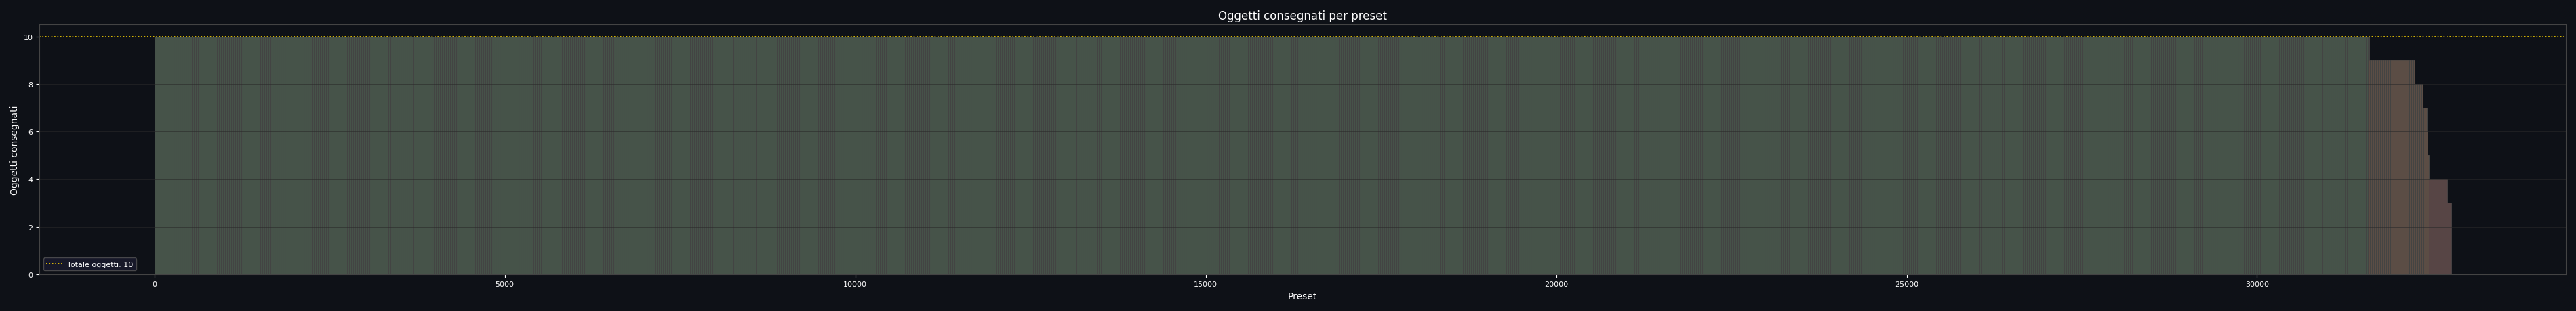
\includegraphics[width=\textwidth]{../../benchmarks/A/32k_sim/Images/plot/grafico_oggetti_consegnati.png}
  \caption{Mappa~A --- 32k sim: distribuzione degli oggetti consegnati per preset. Tasso di completamento: 96,4\%}
  \label{fig:A32k-oggetti}
\end{figure}

\begin{figure}[H]
  \centering
  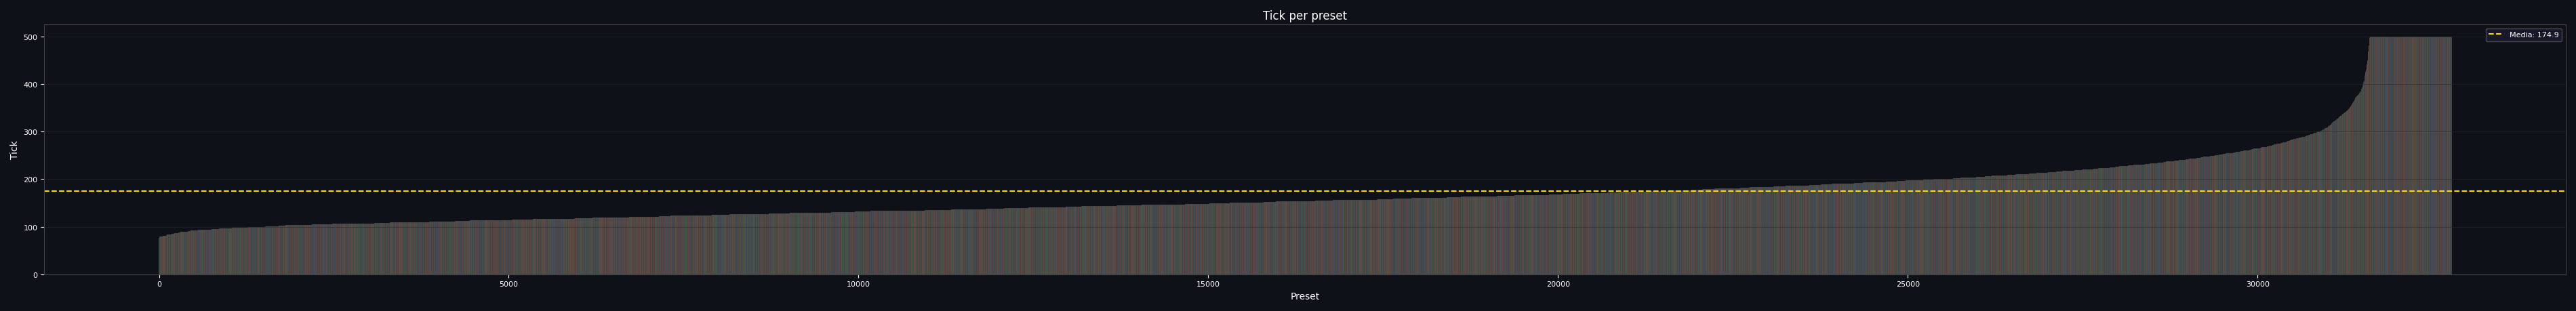
\includegraphics[width=\textwidth]{../../benchmarks/A/32k_sim/Images/plot/grafico_tick_completamento.png}
  \caption{Mappa~A --- 32k sim: tick di completamento per preset. Tick medi: 174,9. Energia media consumata: 173,1 unit\`a.}
  \label{fig:A32k-tick}
\end{figure}

\begin{figure}[H]
  \centering
  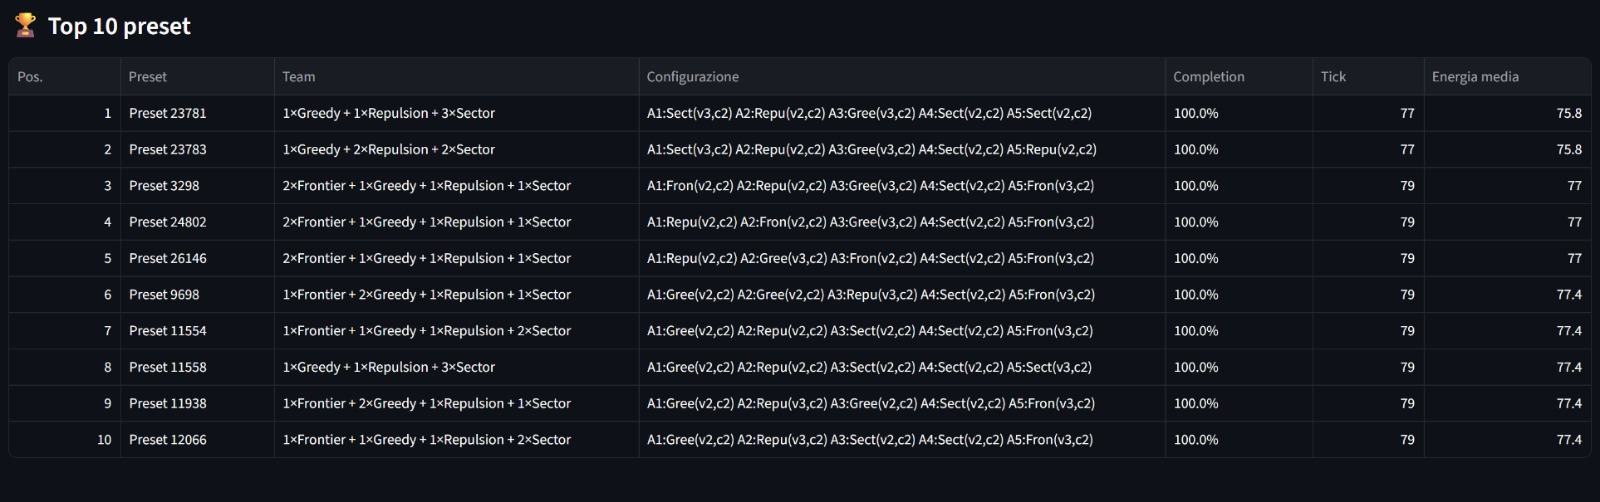
\includegraphics[width=0.92\textwidth]{../../benchmarks/A/32k_sim/Images/tabelle/tabellaTop10.jpeg}
  \caption{Mappa~A --- 32k sim: classifica dei 10 migliori preset per tick di completamento.}
  \label{fig:A32k-top10}
\end{figure}

\begin{table}[H]
\centering
\caption{Mappa~A --- Top~10 preset nel test esaustivo (32k simulazioni).}
\label{tab:A32k-top10}
\small
\begin{tabular}{c l l c c}
\toprule
\textbf{\#} & \textbf{Preset} & \textbf{Composizione team} & \textbf{Tick} & $\overline{E}$ \\
\midrule
1  & 23781 & Sect($v_3$) Repu($v_2$) Gree($v_3$) Sect($v_2$) Sect($v_2$) & 77  & 75{,}8  \\
2  & 23783 & Sect($v_3$) Repu($v_2$) Gree($v_3$) Sect($v_2$) Repu($v_2$) & 77  & 75{,}8  \\
3  & 3298  & Fron($v_2$) Repu($v_2$) Gree($v_3$) Sect($v_2$) Fron($v_3$) & 79  & 77{,}0  \\
4  & 24802 & Repu($v_2$) Fron($v_2$) Gree($v_3$) Sect($v_2$) Fron($v_3$) & 79  & 77{,}0  \\
5  & 26146 & Repu($v_2$) Gree($v_3$) Fron($v_2$) Sect($v_2$) Fron($v_3$) & 79  & 77{,}0  \\
6  & 9698  & Gree($v_2$) Gree($v_2$) Repu($v_3$) Sect($v_2$) Fron($v_3$) & 79  & 77{,}4  \\
7  & 11554 & Gree($v_2$) Repu($v_2$) Sect($v_2$) Sect($v_2$) Fron($v_3$) & 79  & 77{,}4  \\
8  & 11558 & Gree($v_2$) Repu($v_2$) Sect($v_2$) Sect($v_2$) Sect($v_3$) & 79  & 77{,}4  \\
9  & 11938 & Gree($v_2$) Repu($v_3$) Gree($v_2$) Sect($v_2$) Fron($v_3$) & 79  & 77{,}4  \\
10 & 12066 & Gree($v_2$) Repu($v_3$) Sect($v_2$) Sect($v_2$) Fron($v_3$) & 79  & 77{,}4  \\
\bottomrule
\end{tabular}

\vspace{4pt}
{\footnotesize Legenda: Fron = Frontier, Gree = Greedy, Sect = Sector,
Repu = Repulsion. $v_k$ = raggio di visibilit\`a $k$. $c_r = 2$ per tutti.}
\end{table}

%% ── 100×3 ────────────────────────────────────────────────────────────────────
\subsection{Test randomizzato --- 100$\times$3 seed}

La media complessiva sui tre seed \`e:

\begin{itemize}
  \item \textbf{Tasso di completamento medio}: 99,6\,\% (96/100 completati per seed~42 e 44, 97/100 per seed~43).
  \item \textbf{Tick medi di completamento}: $\overline{T} = 158{,}5$ tick
        (media dei preset completati al 100\,\% sui tre seed).
  \item \textbf{Energia media}: $\overline{E} = 169{,}0$.
\end{itemize}

\begin{figure}[H]
  \centering
  \includegraphics[width=0.75\textwidth]{../../benchmarks/A/100_sim/Configurazione.png}
  \caption{Configurazione della Mappa~A utilizzata nel test randomizzato.}
  \label{fig:confA-100}
\end{figure}

\subsubsection*{Seed 42}

\begin{figure}[H]
  \centering
  \includegraphics[width=\textwidth]{../../benchmarks/A/100_sim/seed42/Images/plot/grafico_oggetti_consegnati.png}
  \caption{Mappa~A --- seed 42: oggetti consegnati per preset.}
  \label{fig:As42-oggetti}
\end{figure}

\begin{figure}[H]
  \centering
  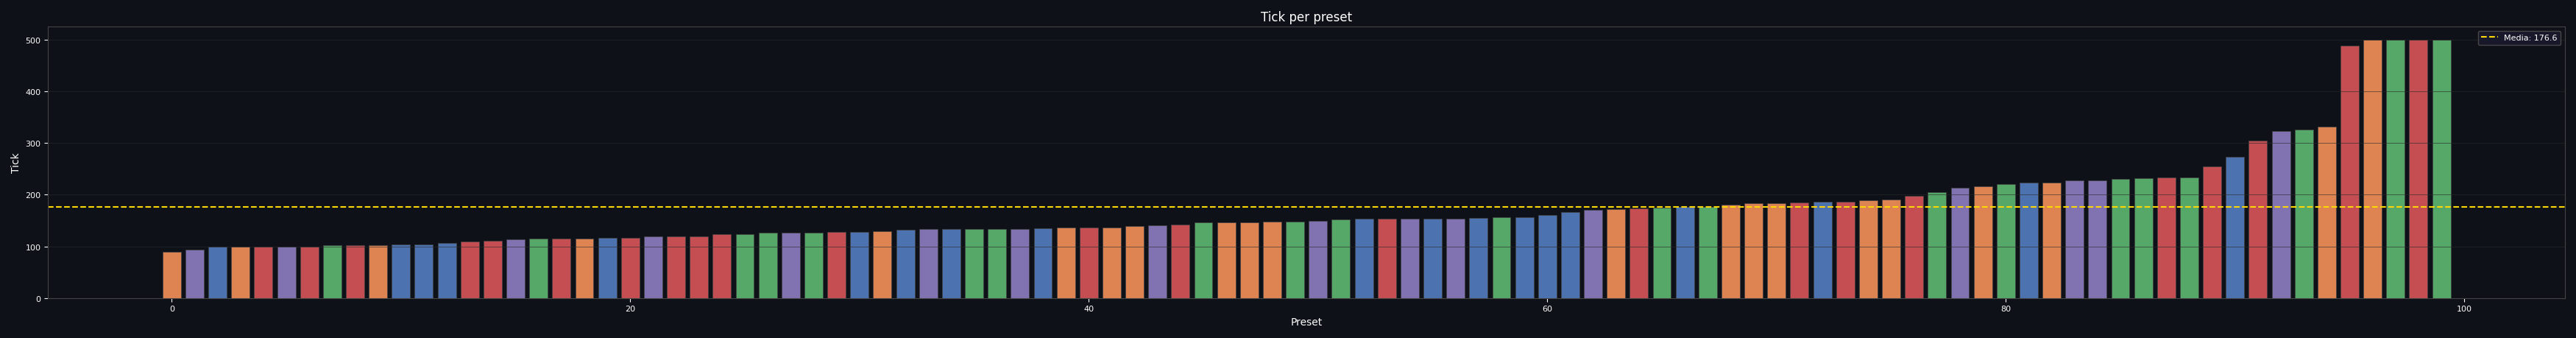
\includegraphics[width=\textwidth]{../../benchmarks/A/100_sim/seed42/Images/plot/grafico_tick_completamento.png}
  \caption{Mappa~A --- seed 42: tick di completamento per preset.}
  \label{fig:As42-tick}
\end{figure}

\begin{figure}[H]
  \centering
  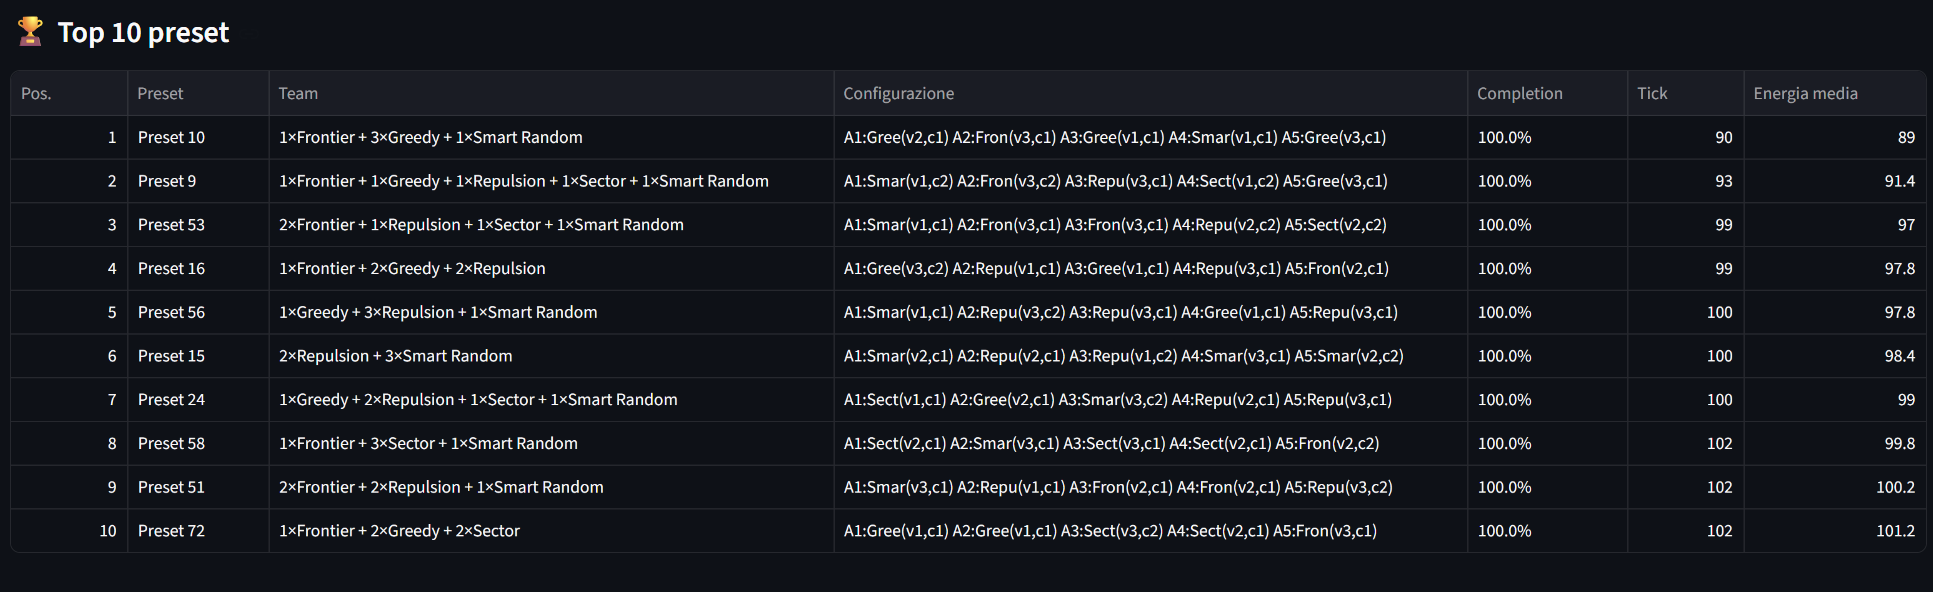
\includegraphics[width=0.92\textwidth]{../../benchmarks/A/100_sim/seed42/Images/tabelle/tabellaTop10.png}
  \caption{Mappa~A --- seed 42: classifica Top~10.}
  \label{fig:As42-top10}
\end{figure}

\subsubsection*{Seed 43}

\begin{figure}[H]
  \centering
  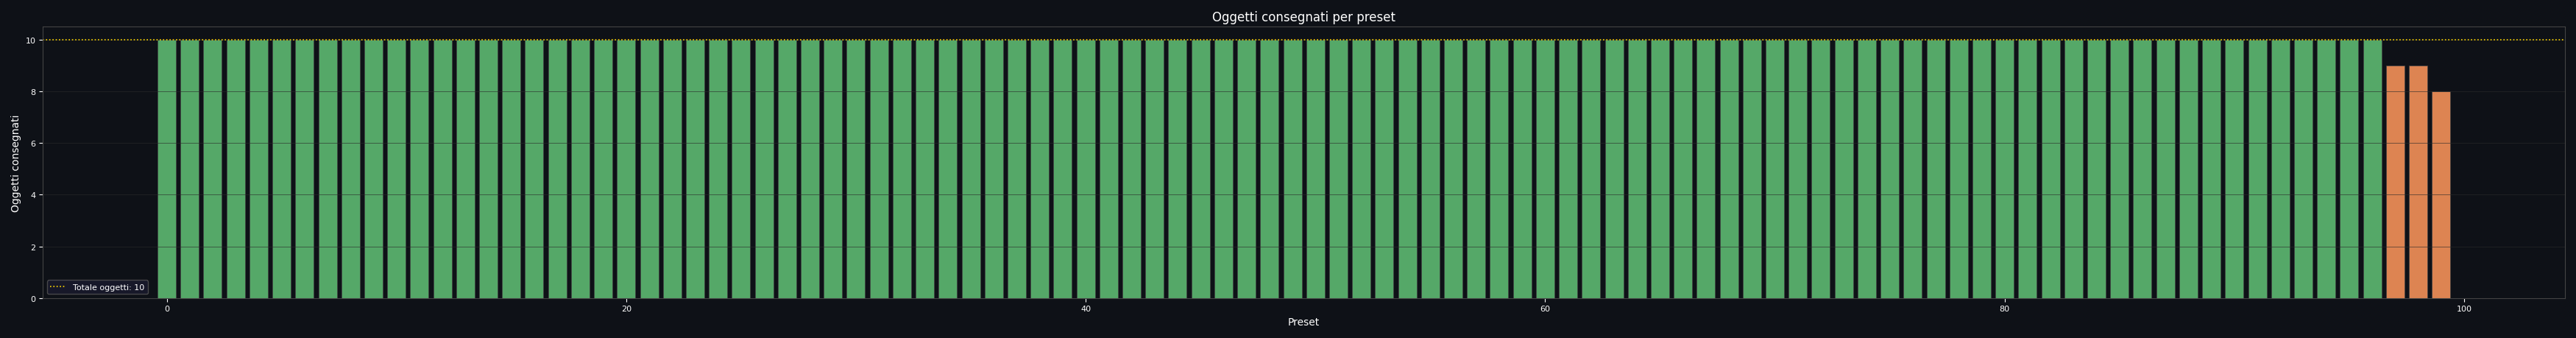
\includegraphics[width=\textwidth]{../../benchmarks/A/100_sim/seed43/Images/plot/grafico_oggetti_consegnati.png}
  \caption{Mappa~A --- seed 43: oggetti consegnati per preset.}
  \label{fig:As43-oggetti}
\end{figure}

\begin{figure}[H]
  \centering
  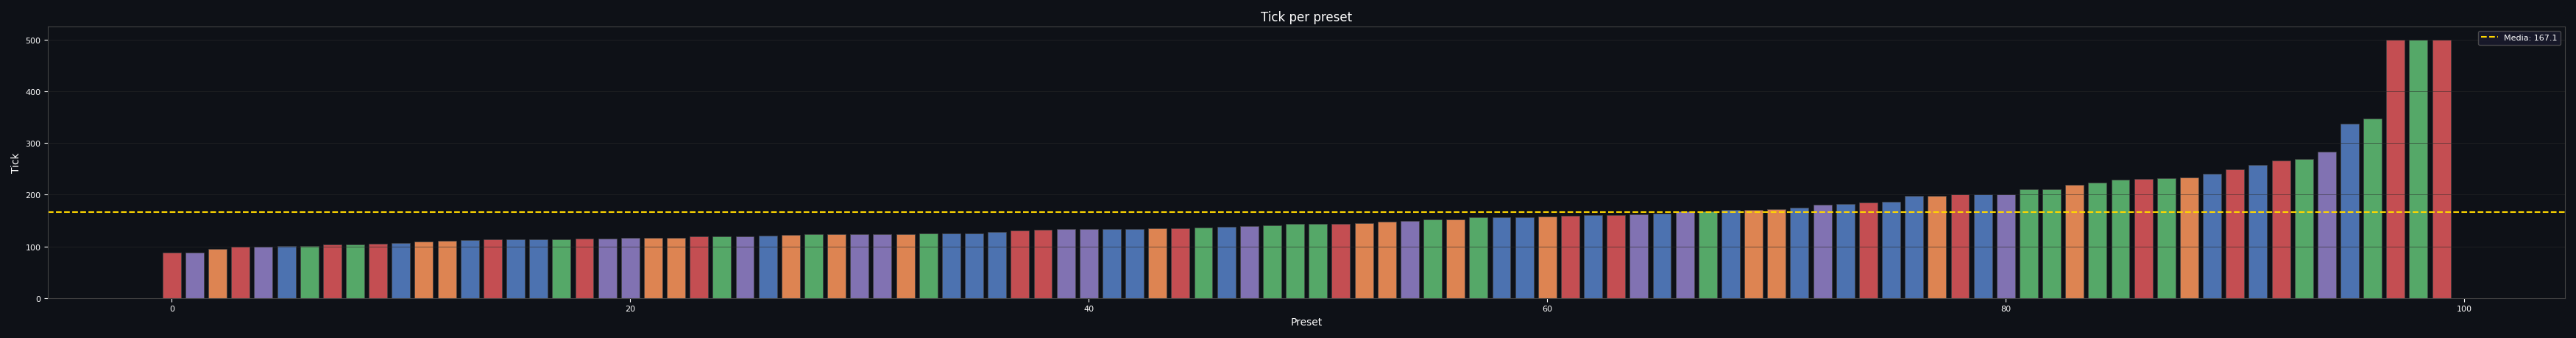
\includegraphics[width=\textwidth]{../../benchmarks/A/100_sim/seed43/Images/plot/grafico_tick_completamento.png}
  \caption{Mappa~A --- seed 43: tick di completamento per preset.}
  \label{fig:As43-tick}
\end{figure}

\begin{figure}[H]
  \centering
  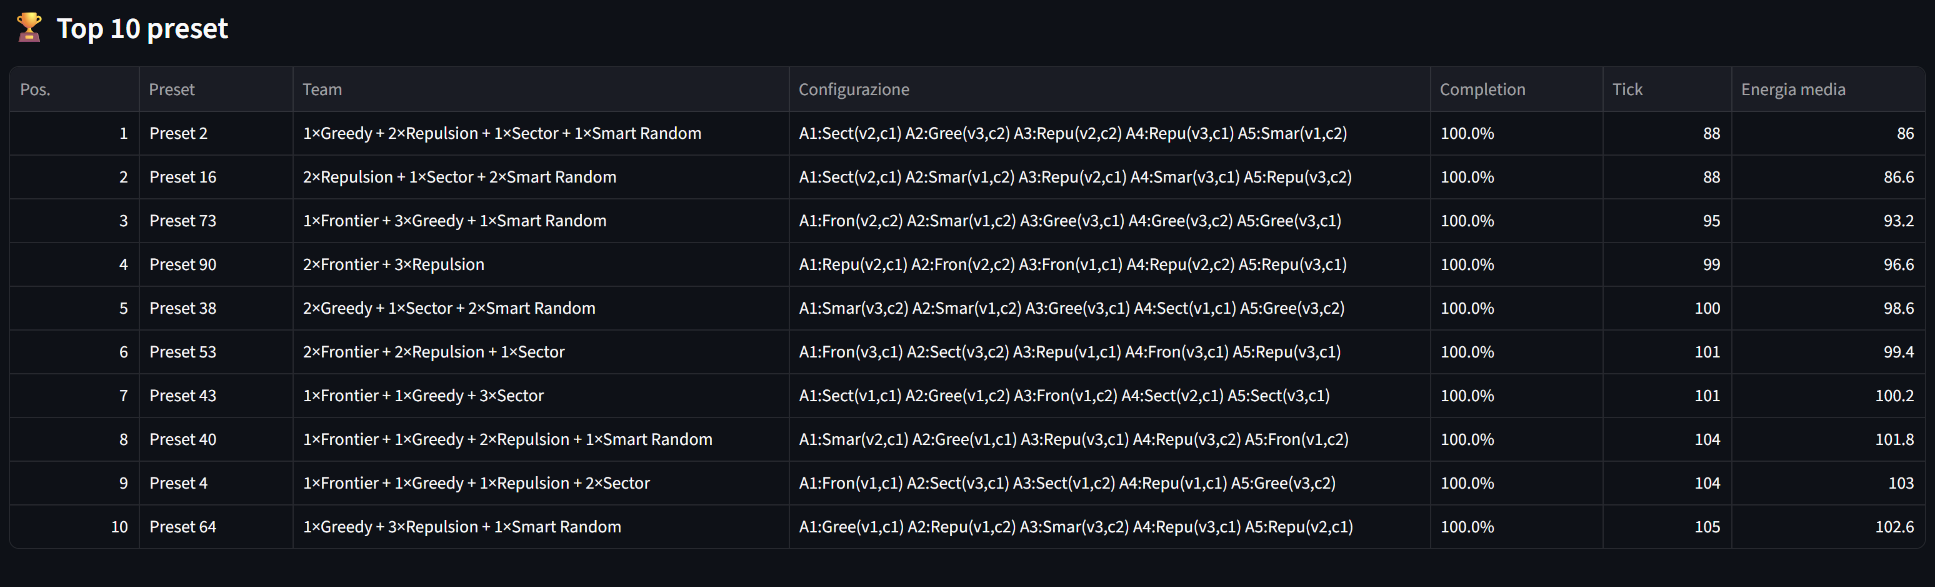
\includegraphics[width=0.92\textwidth]{../../benchmarks/A/100_sim/seed43/Images/tabelle/tabellaTop10.png}
  \caption{Mappa~A --- seed 43: classifica Top~10.}
  \label{fig:As43-top10}
\end{figure}

\subsubsection*{Seed 44}

\begin{figure}[H]
  \centering
  \includegraphics[width=\textwidth]{../../benchmarks/A/100_sim/seed44/Images/plot/grafico_oggetti_consegnati.png}
  \caption{Mappa~A --- seed 44: oggetti consegnati per preset.}
  \label{fig:As44-oggetti}
\end{figure}

\begin{figure}[H]
  \centering
  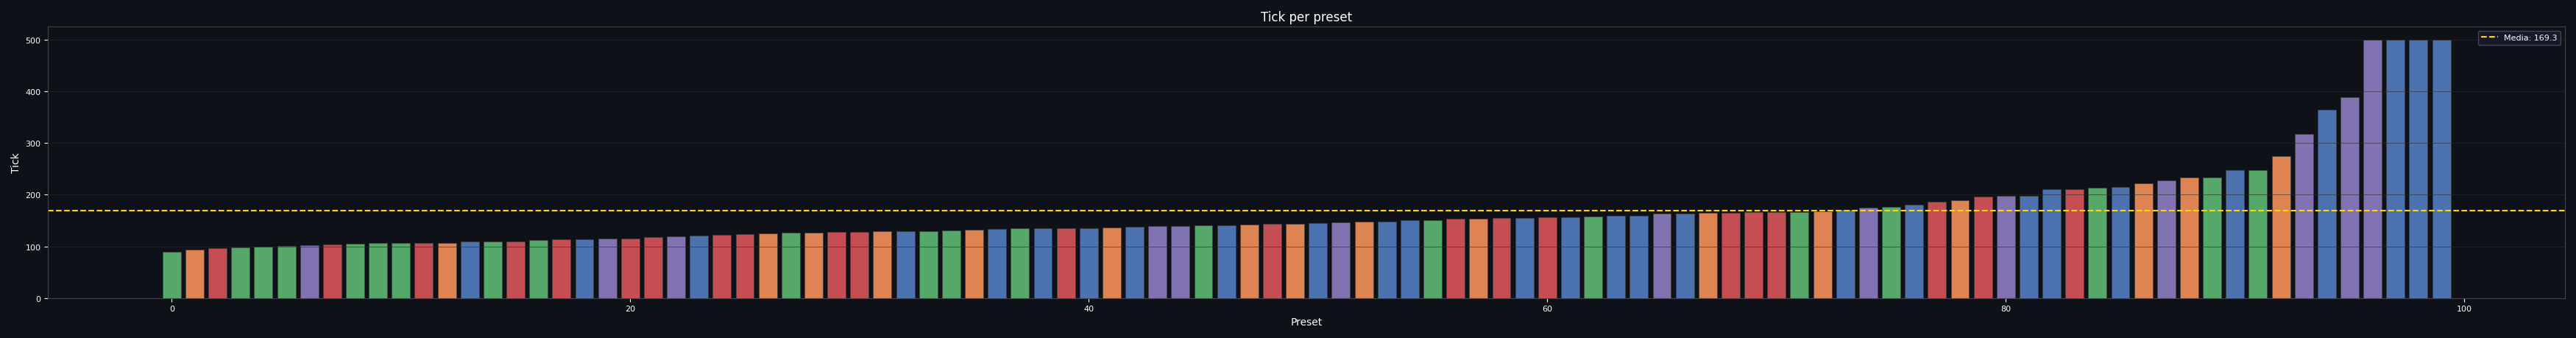
\includegraphics[width=\textwidth]{../../benchmarks/A/100_sim/seed44/Images/plot/grafico_tick_completamento.png}
  \caption{Mappa~A --- seed 44: tick di completamento per preset.}
  \label{fig:As44-tick}
\end{figure}

\begin{figure}[H]
  \centering
  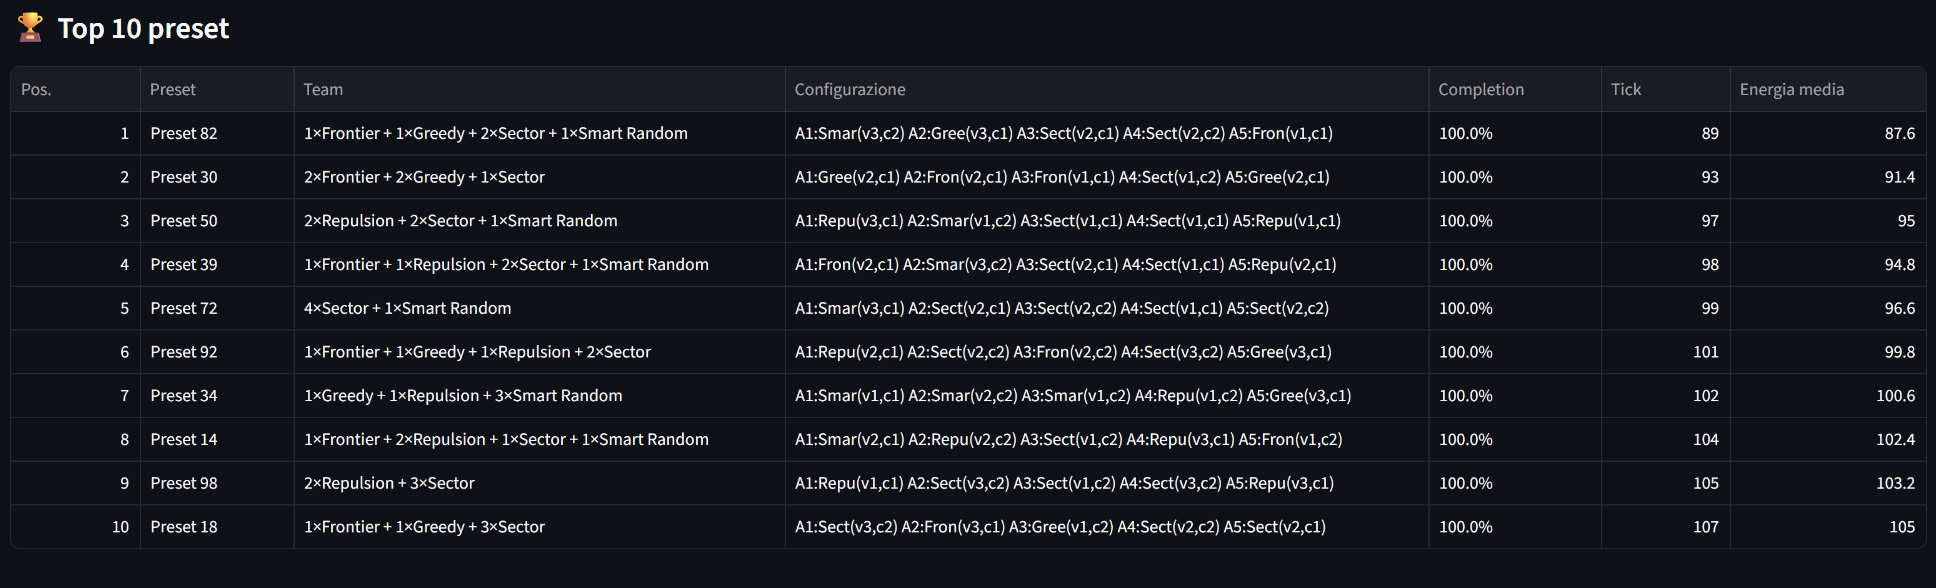
\includegraphics[width=0.92\textwidth]{../../benchmarks/A/100_sim/seed44/Images/tabelle/tabellaTop10.png}
  \caption{Mappa~A --- seed 44: classifica Top~10.}
  \label{fig:As44-top10}
\end{figure}

%% ═════════════════════════════════════════════════════════════════════════════
\section{Mappa B}
%% ═════════════════════════════════════════════════════════════════════════════

\subsection{Test esaustivo --- 32.768 simulazioni}

Tempo CPU totale: circa 2\,h\,30\,min.

\begin{itemize}
  \item \textbf{Tasso di completamento}: 99,6\,\% (32.652 su 32.768).
        $\overline{r} = 0{,}9995$.
  \item \textbf{Tick medi di completamento}: $\overline{T} = 105{,}7$ tick.
        Il miglior preset ha completato in 57 tick.
  \item \textbf{Energia media}: $\overline{E} = 104{,}7$.
\end{itemize}

Rispetto alla Mappa~A, la Mappa~B risulta sensibilmente pi\`u
facile: tasso di completamento pi\`u alto (+3,2~pp), tick medi pi\`u
bassi ($-35\,\%$) e minor consumo energetico ($-40\,\%$).

\begin{figure}[H]
  \centering
  \includegraphics[width=0.75\textwidth]{../../benchmarks/B/32k_sim/Configurazione.png}
  \caption{Configurazione della Mappa~B utilizzata nel test esaustivo.}
  \label{fig:confB-32k}
\end{figure}

\begin{figure}[H]
  \centering
  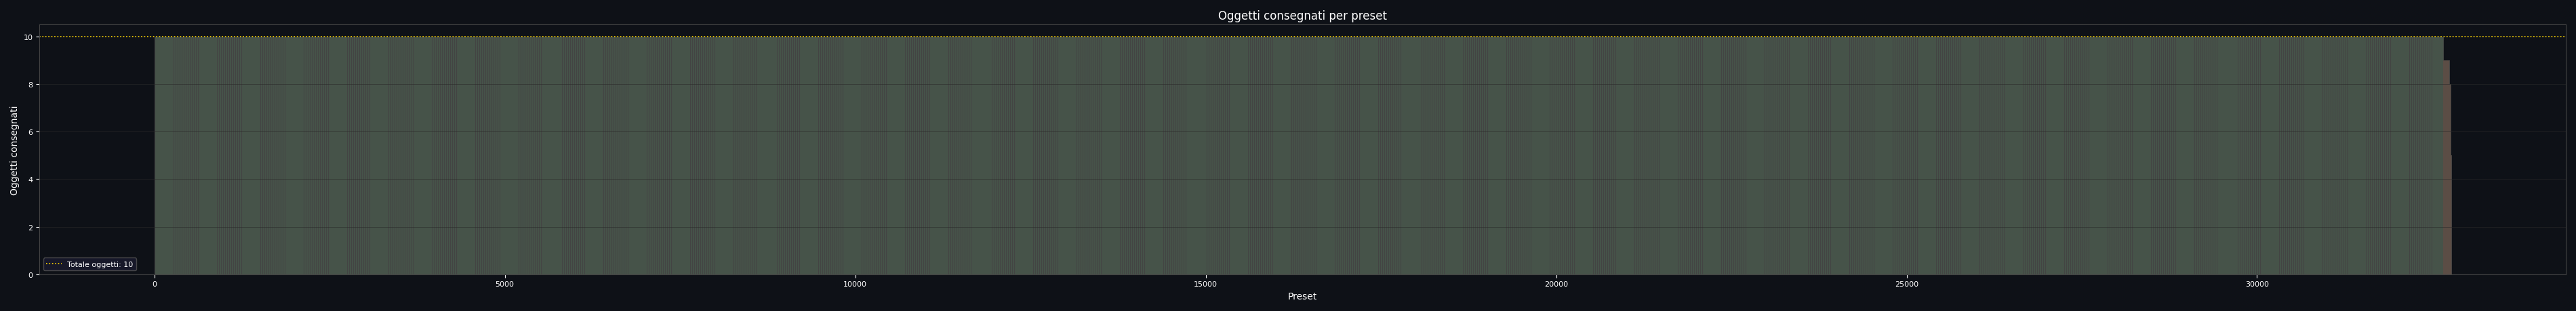
\includegraphics[width=\textwidth]{../../benchmarks/B/32k_sim/Images/plot/grafico_oggetti_consegnati.png}
  \caption{Mappa~B --- 32k sim: distribuzione degli oggetti consegnati per preset. Tasso di completamento: 99,6\%}
  \label{fig:B32k-oggetti}
\end{figure}

\begin{figure}[H]
  \centering
  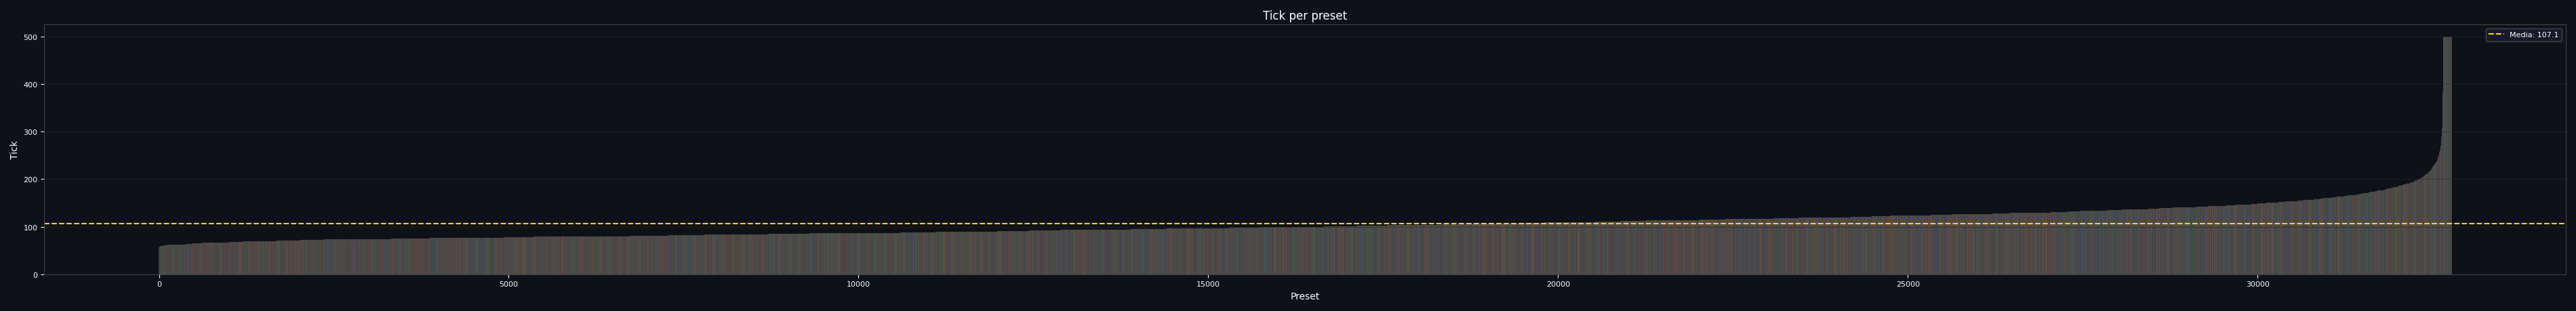
\includegraphics[width=\textwidth]{../../benchmarks/B/32k_sim/Images/plot/grafico_tick_completamento.png}
  \caption{Mappa~B --- 32k sim: tick di completamento per preset. Tick medi: 107,1. Energia media consumata: 104,7 unit\`a.}
  \label{fig:B32k-tick}
\end{figure}

\begin{figure}[H]
  \centering
  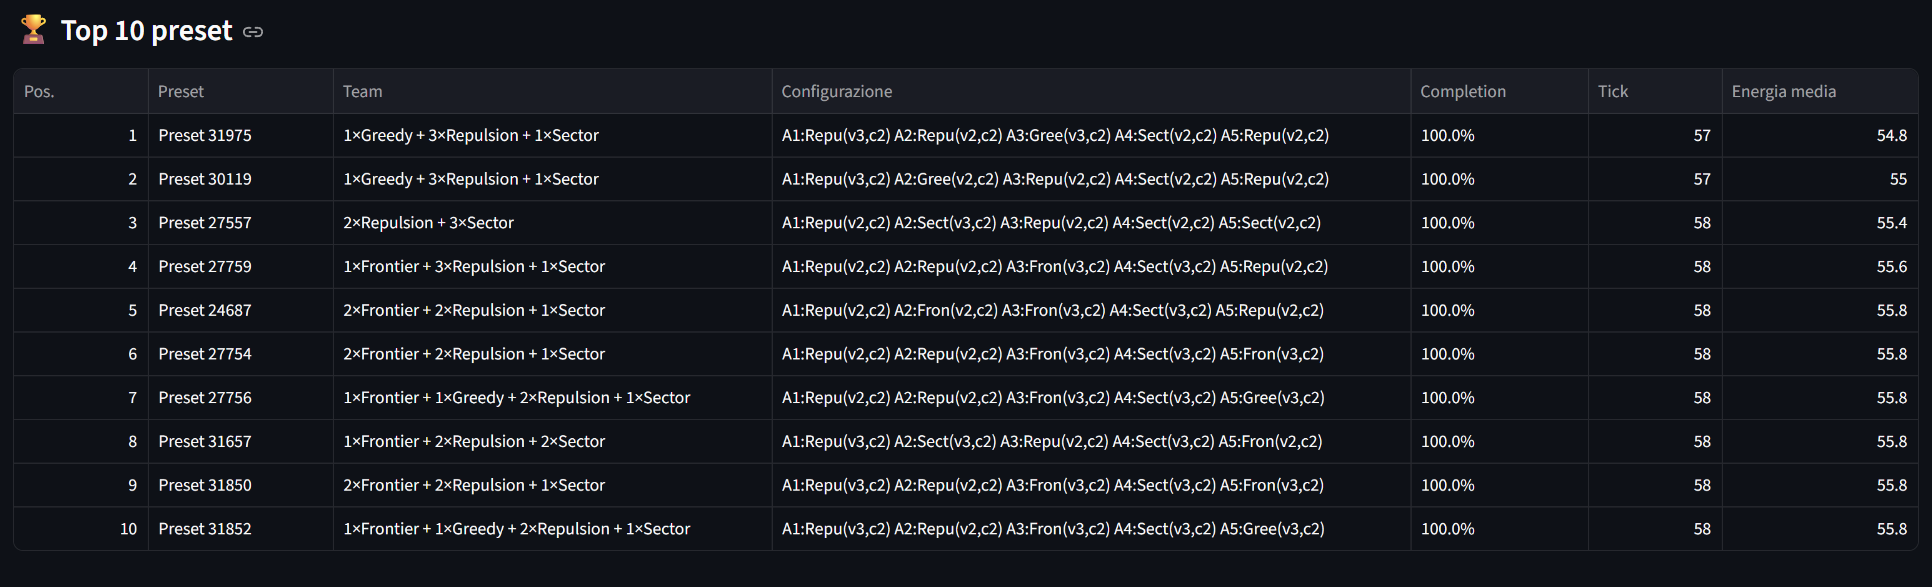
\includegraphics[width=0.92\textwidth]{../../benchmarks/B/32k_sim/Images/tabelle/tabellaTop10.png}
  \caption{Mappa~B --- 32k sim: classifica dei 10 migliori preset per tick di completamento.}
  \label{fig:B32k-top10}
\end{figure}

\begin{table}[H]
\centering
\caption{Mappa~B --- Top~10 preset nel test esaustivo (32k simulazioni).}
\label{tab:B32k-top10}
\small
\begin{tabular}{c l l c c}
\toprule
\textbf{\#} & \textbf{Preset} & \textbf{Composizione team} & \textbf{Tick} & $\overline{E}$ \\
\midrule
1  & 31975 & Repu($v_3$) Repu($v_2$) Gree($v_3$) Sect($v_2$) Repu($v_2$) & 57  & 54{,}8  \\
2  & 30119 & Repu($v_3$) Gree($v_2$) Repu($v_2$) Sect($v_2$) Repu($v_2$) & 57  & 55{,}0  \\
3  & 27557 & Repu($v_2$) Sect($v_3$) Repu($v_2$) Sect($v_2$) Sect($v_2$) & 58  & 55{,}4  \\
4  & 27759 & Repu($v_2$) Repu($v_2$) Fron($v_3$) Sect($v_3$) Repu($v_2$) & 58  & 55{,}6  \\
5  & 24687 & Repu($v_2$) Fron($v_2$) Fron($v_3$) Sect($v_3$) Repu($v_2$) & 58  & 55{,}8  \\
6  & 27754 & Repu($v_2$) Repu($v_2$) Fron($v_3$) Sect($v_3$) Fron($v_3$) & 58  & 55{,}8  \\
7  & 27756 & Repu($v_2$) Repu($v_2$) Fron($v_3$) Sect($v_3$) Gree($v_3$) & 58  & 55{,}8  \\
8  & 31657 & Repu($v_3$) Sect($v_3$) Repu($v_2$) Sect($v_3$) Fron($v_2$) & 58  & 55{,}8  \\
9  & 31850 & Repu($v_3$) Repu($v_2$) Fron($v_3$) Sect($v_3$) Fron($v_3$) & 58  & 55{,}8  \\
10 & 31852 & Repu($v_3$) Repu($v_2$) Fron($v_3$) Sect($v_3$) Gree($v_3$) & 58  & 55{,}8  \\
\bottomrule
\end{tabular}

\vspace{4pt}
{\footnotesize Legenda: Fron = Frontier, Gree = Greedy, Sect = Sector,
Repu = Repulsion. $v_k$ = raggio di visibilit\`a $k$. $c_r = 2$ per tutti.}
\end{table}

%% ── 100×3 ────────────────────────────────────────────────────────────────────
\subsection{Test randomizzato --- 100$\times$3 seed}

La media complessiva sui tre seed \`e:

\begin{itemize}
  \item \textbf{Tasso di completamento medio}: 99,97\,\% (tutti i 100 preset completati
        con seed~42 e 43; 99/100 con seed~44).
  \item \textbf{Tick medi di completamento}: $\overline{T} = 112{,}6$ tick.
  \item \textbf{Energia media}: $\overline{E} = 111{,}6$.
\end{itemize}

\begin{figure}[H]
  \centering
  \includegraphics[width=0.75\textwidth]{../../benchmarks/B/100_sim/Configurazione.png}
  \caption{Configurazione della Mappa~B utilizzata nel test randomizzato.}
  \label{fig:confB-100}
\end{figure}

\subsubsection*{Seed 42}

\begin{figure}[H]
  \centering
  \includegraphics[width=\textwidth]{../../benchmarks/B/100_sim/seed42/Images/plot/grafico_oggetti_consegnati.png}
  \caption{Mappa~B --- seed 42: oggetti consegnati per preset.}
  \label{fig:Bs42-oggetti}
\end{figure}

\begin{figure}[H]
  \centering
  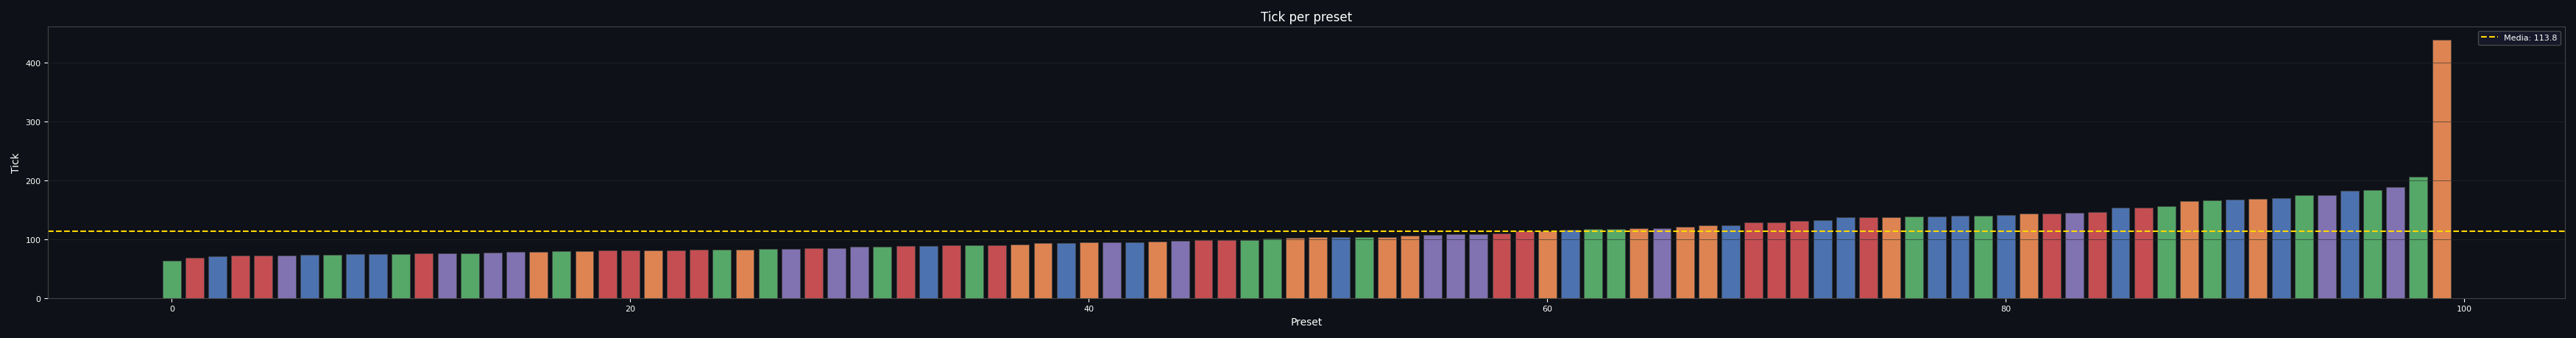
\includegraphics[width=\textwidth]{../../benchmarks/B/100_sim/seed42/Images/plot/grafico_tick_completamento.png}
  \caption{Mappa~B --- seed 42: tick di completamento per preset.}
  \label{fig:Bs42-tick}
\end{figure}

\begin{figure}[H]
  \centering
  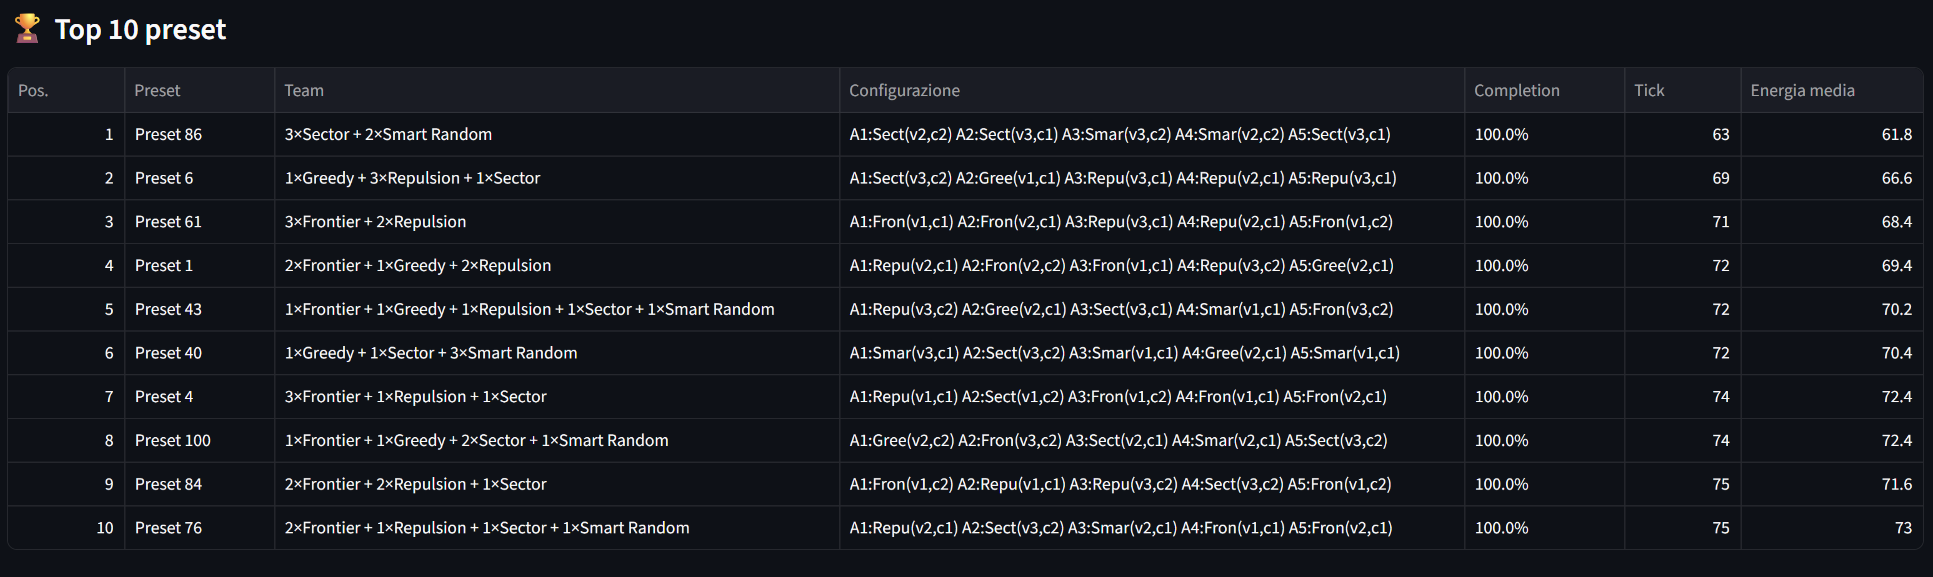
\includegraphics[width=0.92\textwidth]{../../benchmarks/B/100_sim/seed42/Images/tabelle/tabellaTop10.png}
  \caption{Mappa~B --- seed 42: classifica Top~10.}
  \label{fig:Bs42-top10}
\end{figure}

\subsubsection*{Seed 43}

\begin{figure}[H]
  \centering
  \includegraphics[width=\textwidth]{../../benchmarks/B/100_sim/seed43/Images/plot/grafico_oggetti_consegnati.png}
  \caption{Mappa~B --- seed 43: oggetti consegnati per preset.}
  \label{fig:Bs43-oggetti}
\end{figure}

\begin{figure}[H]
  \centering
  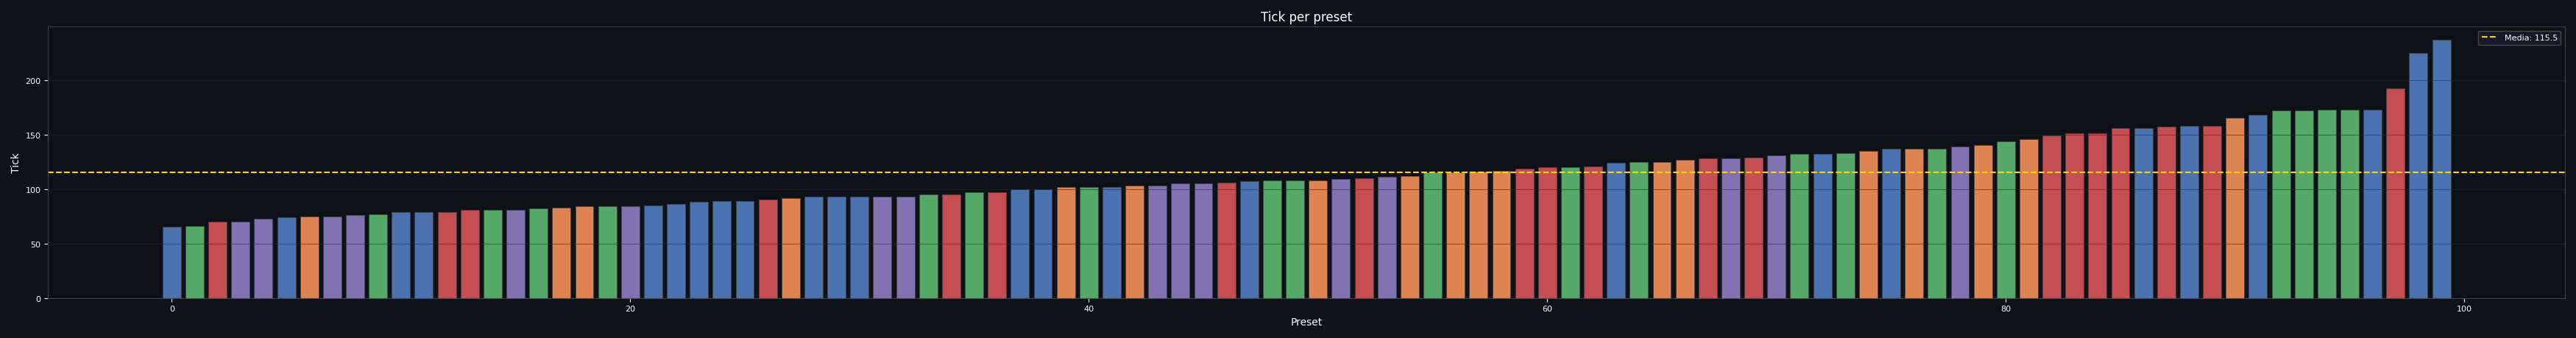
\includegraphics[width=\textwidth]{../../benchmarks/B/100_sim/seed43/Images/plot/grafico_tick_completamento.png}
  \caption{Mappa~B --- seed 43: tick di completamento per preset.}
  \label{fig:Bs43-tick}
\end{figure}

\begin{figure}[H]
  \centering
  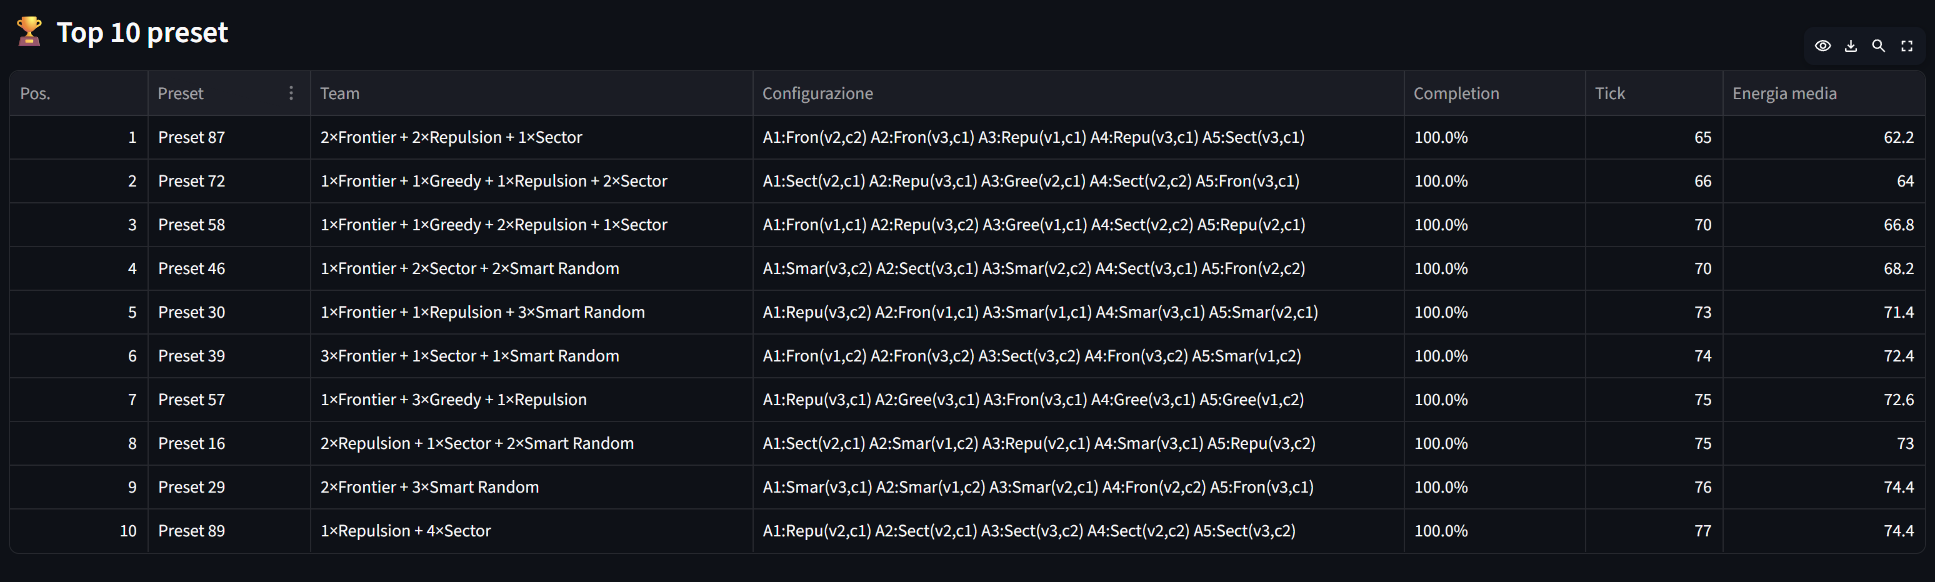
\includegraphics[width=0.92\textwidth]{../../benchmarks/B/100_sim/seed43/Images/tabelle/tabellaTop10.png}
  \caption{Mappa~B --- seed 43: classifica Top~10.}
  \label{fig:Bs43-top10}
\end{figure}

\subsubsection*{Seed 44}

\begin{figure}[H]
  \centering
  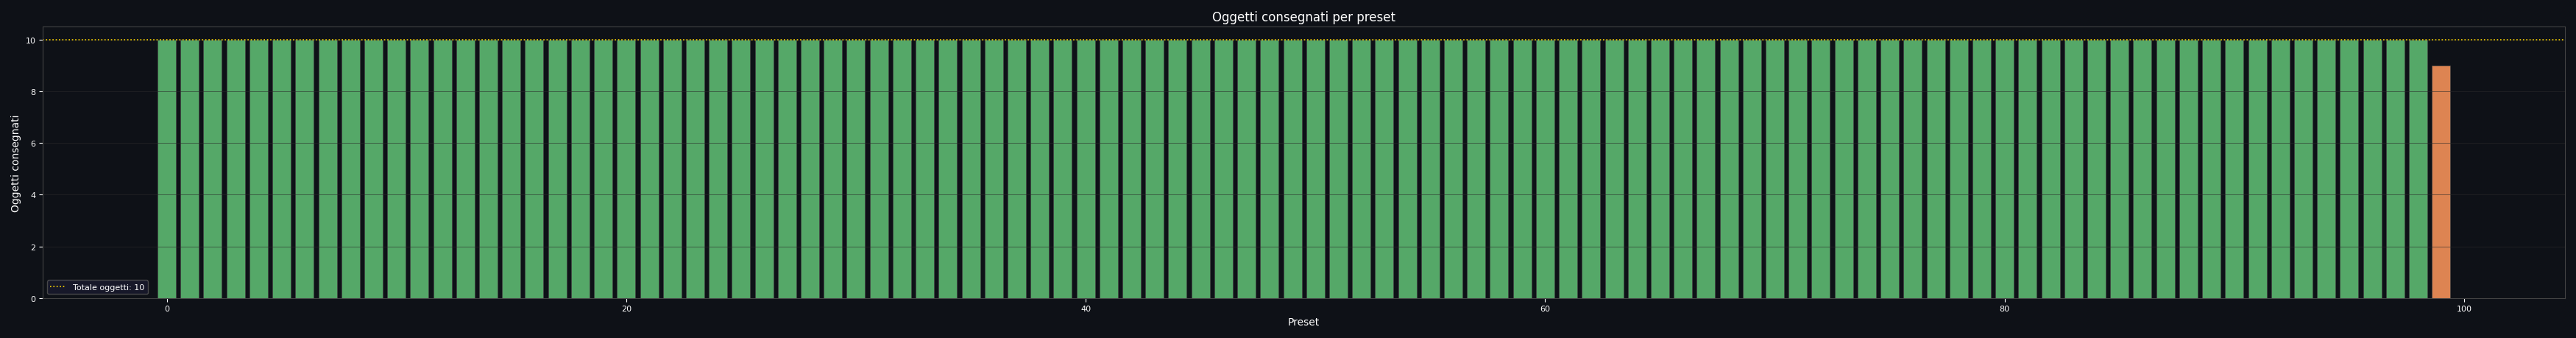
\includegraphics[width=\textwidth]{../../benchmarks/B/100_sim/seed44/Images/plot/grafico_oggetti_consegnati.png}
  \caption{Mappa~B --- seed 44: oggetti consegnati per preset.}
  \label{fig:Bs44-oggetti}
\end{figure}

\begin{figure}[H]
  \centering
  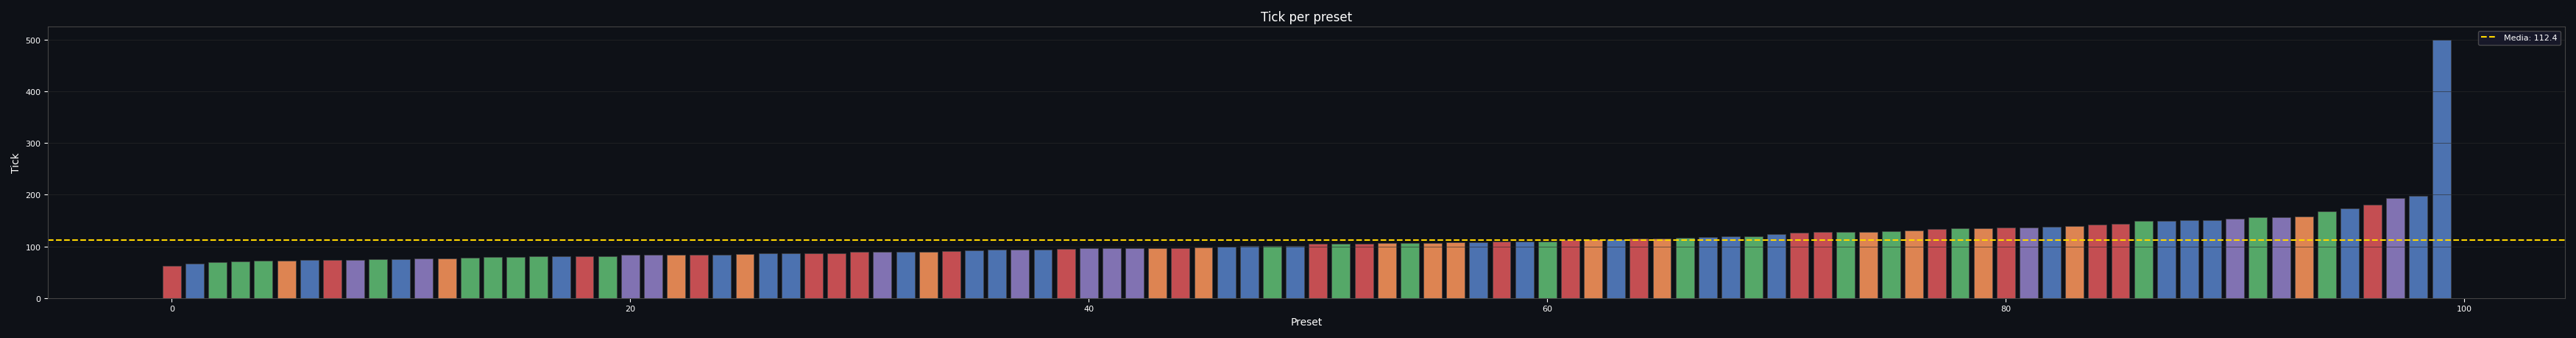
\includegraphics[width=\textwidth]{../../benchmarks/B/100_sim/seed44/Images/plot/grafico_tick_completamento.png}
  \caption{Mappa~B --- seed 44: tick di completamento per preset.}
  \label{fig:Bs44-tick}
\end{figure}

\begin{figure}[H]
  \centering
  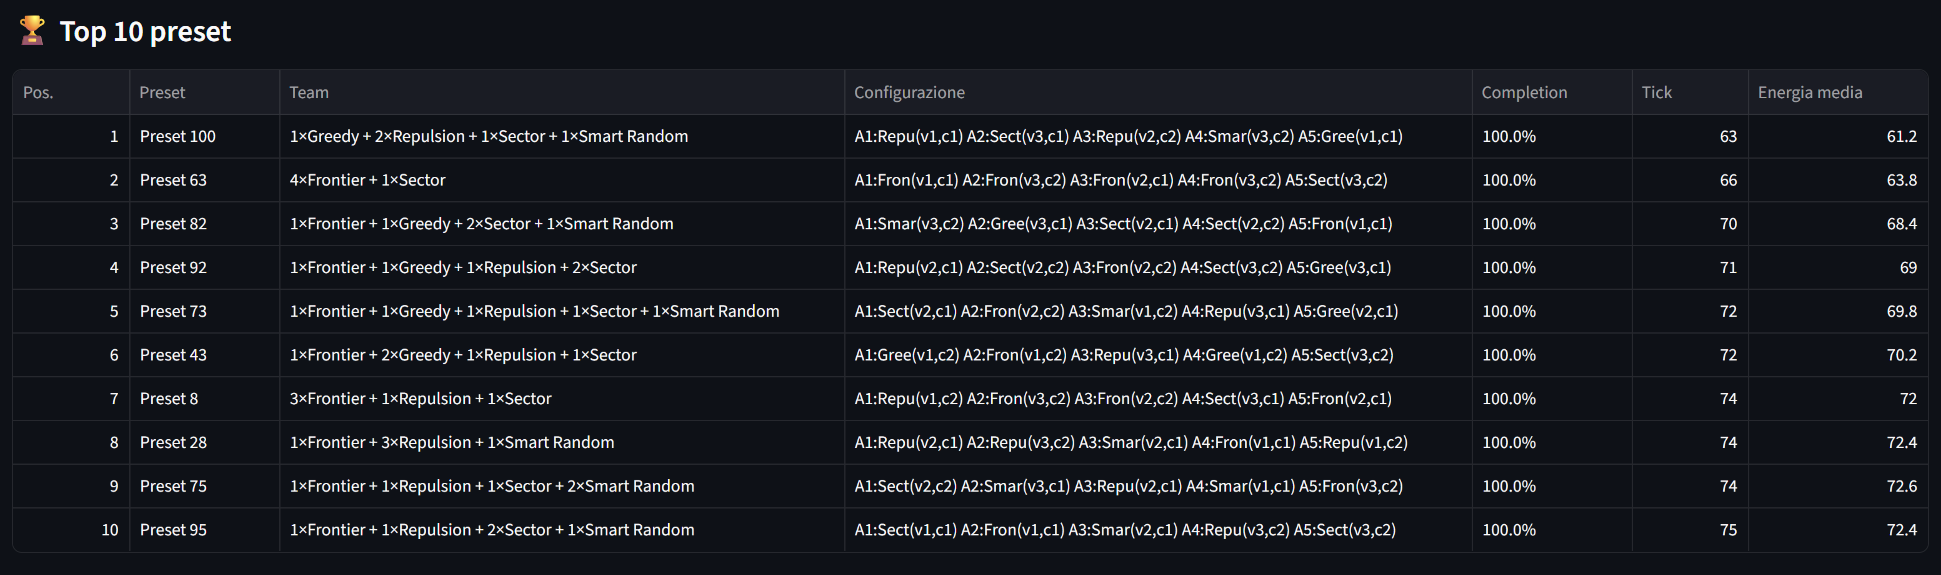
\includegraphics[width=0.92\textwidth]{../../benchmarks/B/100_sim/seed44/Images/tabelle/tabellaTop10.png}
  \caption{Mappa~B --- seed 44: classifica Top~10.}
  \label{fig:Bs44-top10}
\end{figure}

%% ═════════════════════════════════════════════════════════════════════════════
\section{Considerazioni sui risultati}
%% ═════════════════════════════════════════════════════════════════════════════

\subsection{Confronto tra le due mappe}

La Mappa~B risulta sistematicamente pi\`u semplice della Mappa~A su tutte le metriche.
Nel test esaustivo il miglior preset completa in 57~tick (contro i 77 della Mappa~A),
con un tick medio di completamento di 105{,}7 contro 162{,}9 ($-35\,\%$) e un consumo
energetico medio di 103{,}3 contro 161{,}1 ($-36\,\%$).
Il tasso di completamento sale dal 96{,}4\,\% al 99{,}6\,\%.
Questa differenza \`e attribuibile alla topologia della mappa:
una pianta pi\`u aperta riduce i cammini medi agente-oggetto e agente-magazzino,
abbassando sia i tick sia l'energia necessari.

\subsection{Impatto della strategia dominante}

Analizzando i 32.768 preset completati per strategia dominante
(la strategia che compare pi\`u volte nel team di 5 agenti), emerge una chiara
differenza tra le due mappe:

\begin{itemize}
  \item \textbf{Mappa~A}: le quattro strategie ottengono tick medi molto simili
        (Repulsion 158{,}7, Greedy 161{,}5, Sector 163{,}0, Frontier 168{,}5),
        con Repulsion leggermente avvantaggiata.
        Nella Top~10, Sector domina con 17 assegnazioni su 50, seguito da
        Greedy~(12) e Repulsion~(11).
    \item \textbf{Mappa~B}: Repulsion emerge nettamente come strategia migliore
      (101{,}5 tick medi, $-9\,\%$ rispetto a Frontier).
        Nella Top~10 compare 23 volte su 50, contro 13 di Sector e 10 di Frontier.
\end{itemize}

\textit{Nota sulla posizione sistemática di Sector nei team Top~10:}
Sector appare sistematicamente inserito in 4\textsuperscript{a} posizione
(indice agente 3) nei team Top~10 di entrambe le mappe. Questo fenomeno non \`e casuale:
la strategia Sector divide la griglia in bande orizzontali assegnate agli agenti in base a
$\texttt{agent\_id} \bmod N$. Agenti con ID inferiore occupano bande pi\`u alte e procedono
verso il basso in modo sistematico. Posizionare Sector in 4\textsuperscript{a} posizione
minimizza la sovrapposizione con gli altri agenti: se Sector avesse ID inferiore,
la sua banda occuperrebbe spazio sin dall'inizio della mappa, potenzialmente entrando
in conflitto con le traiettorie delle altre strategie. Questa configurazione emerge
naturalmente dall'ottimizzazione, riflettendo il trade-off tra copertura sistematica
di Sector e flessibilità delle altre strategie nei team misti.

\subsection{Team eterogenei vs omogenei}

I team omogenei (tutti e 5 gli agenti con la stessa strategia) rappresentano
solo 128 dei 32.768 preset per ciascuna mappa. I risultati sono eloquenti:

\begin{itemize}
  \item \textbf{Mappa~A}: team omogenei completano nel 96{,}9\,\% dei casi con una media
        di 172{,}5~tick; team eterogenei completano nel 96{,}4\,\% con 162{,}9~tick
        e ottengono il record assoluto di 77~tick. Nessun team omogeneo scende sotto i 99~tick.
  \item \textbf{Mappa~B}: team omogenei completano nel 100\,\% dei casi con 102{,}3~tick
        medi, ma il miglior risultato \`e 64~tick; i team eterogenei raggiungono 57~tick.
\end{itemize}

In entrambe le mappe il \textbf{miglior preset assoluto \`e sempre eterogeneo}. Un team
misto beneficia della complementarit\`a tra le strategie: Sector fornisce copertura
sistematica, Repulsion garantisce dispersione, Greedy ottimizza i percorsi verso i
magazzini e Frontier esplora le zone residue.

\subsection{Impatto del raggio di visibilit\`a}

Raggruppando i preset completati per raggio di visibilit\`a medio del team ($\bar{v}_r$), si
osserva un trend diverso nelle due mappe:

\begin{itemize}
  \item \textbf{Mappa~A}: i tick medi calano da 175{,}1 ($\bar{v}_r=2{,}0$) a 152{,}6
        ($\bar{v}_r=2{,}8$), ma risalgono a 162{,}9 per $\bar{v}_r=3{,}0$.
        Il raggio ottimale si colloca intorno a $\bar{v}_r \approx 2{,}6$--$2{,}8$:
        un campo visivo troppo ampio aumenta il costo computazionale del ray casting
        senza aggiungere informazione utile in corridoi stretti.
  \item \textbf{Mappa~B}: i tick calano monotonicamente da 116{,}1 ($\bar{v}_r=2{,}0$)
        a 96{,}7 ($\bar{v}_r=3{,}0$).
        Su una mappa aperta un raggio maggiore \`e sempre vantaggioso perch\'e
        incrementa direttamente l'area scansionata ad ogni tick.
\end{itemize}

Nonostante queste differenze, i Top~10 di entrambe le mappe mantengono un mix di raggi~2 e~3,
suggerendo che la diversit\`a percettiva nel team contribuisce alla robustezza.

\subsection{Robustezza ai seed casuali}

Il test randomizzato con 3~seed indipendenti consente di stimare la sensibilit\`a al rumore
stocastico. I risultati sono stabili:

\begin{itemize}
  \item \textbf{Mappa~A}: i tick medi oscillano tra 155{,}5 e 163{,}1 nei tre seed,
        con una variazione massima del $\pm 2{,}4\,\%$ rispetto alla media.
        Il tasso di completamento \`e costante ($96$--$97\,\%$).
  \item \textbf{Mappa~B}: i tick oscillano tra 108{,}5 e 115{,}5 ($\pm 3{,}1\,\%$).
        Il completamento \`e quasi perfetto ($99$--$100\,\%$) su tutti e tre i seed.
\end{itemize}

La bassa varianza inter-seed conferma che le prestazioni osservate dipendono prevalentemente
dalla configurazione del team e dalla topologia della mappa, non dalla specifica
distribuzione casuale degli oggetti.

\subsection{Riepilogo}

\begin{enumerate}
  \item La topologia della mappa \`e il fattore pi\`u influente: mappe aperte (B) sono
        risolvibili il 35\,\% pi\`u velocemente di mappe strutturate (A).
  \item I team eterogenei battono sistematicamente quelli omogenei nei tempi migliori,
        sfruttando la complementarit\`a tra strategie diverse.
  \item Repulsion \`e la strategia pi\`u performante su mappe aperte;
        Sector e Greedy risultano competitivi su mappe con corridoi.
  \item Un raggio di visibilit\`a elevato \`e sempre vantaggioso su mappe aperte,
        mentre su mappe strutturate esiste un punto di rendimento decrescente
        intorno a $\bar{v}_r \approx 2{,}6$--$2{,}8$.
  \item Il sistema mostra buona robustezza statistica, con variazioni contenute
        al variare del seed casuale.
\end{enumerate}

\newpage
% ═════════════════════════════════════════════════════════════════════════════
\subsection{Riepilogo delle euristiche utilizzate}
% ═════════════════════════════════════════════════════════════════════════════

Il sistema impiega un insieme composito di euristiche, ciascuna con un ruolo specifico
nel coordinamento e nella decisione dei team multi-agente:

\begin{description}
  \item[\textbf{Ray-casting (Bresenham)}]
        Calcola la visione dell'agente entro raggio $v_r$ considerando l'occlusione
        da muri. Base della percezione distribuita.
  
  \item[\textbf{Coverage targets}]
        Fornisce tre livelli di priorit\`a per l'esplorazione: celle inesplorate,
        celle stale (non visitate di recente), pattugliamento. Guida tutte le strategie
        verso aree di maggior interesse.
  
  \item[\textbf{Guadagno informativo (\textit{info\_gain})}]
        Per una cella candidata~$t$, conta le celle non ancora viste che l'agente
        osserverebbe da quella posizione:
        $$\text{info\_gain}(t) = \bigl|\,\{(r,c) : |r - t_r| + |c - t_c| \le v_r
        \;\wedge\; (r,c) \notin \text{seen\_cells}\}\,\bigr|$$
        Usato da Smart Random Walk e Greedy per favorire mosse verso aree dense
        di celle inesplorate.
  
  \item[\textbf{Scelta dell'ingresso di consegna (Costo dinamico)}]
        Per un ingresso~$e$ combina distanza, congestione e prenotazioni:
        $$C(e) \;=\; d(\text{agent},\,e) \;+\; 4{,}5\cdot Q_{\text{local}}
        \;+\; 1{,}5\cdot R_{\text{reserved}} \;+\; \varepsilon_{\text{tie}}$$
        dove $Q_{\text{local}}$ sono gli agenti noti entro raggio~2 e $R_{\text{reserved}}$
        \`e il numero di prenotazioni attive. Scelta rideterminata a ogni tick, con hysteresis
        del 20\% per evitare oscillazioni.
  
  \item[\textbf{Separazione (Repulsion)}]
        Massimizza la distanza media dagli agenti noti:
        $$\text{score}(t) = \frac{1}{|\mathcal{A}|}\sum_{a \in \mathcal{A}} d(t, a) - d(\text{agent}, t)$$
        Induce dispersione naturale senza comunicazione esplicita; efficace su mappe aperte.
  
  \item[\textbf{Frontiere (\textit{frontier-based})}]
        Identifica celle visitate che confinano con celle non visitate. Classico
        approccio all'esplorazione sistematica con A* per il raggiungimento.
  
  \item[\textbf{Costo composito (Greedy)}]
        Minimizza il costo composito di esplorazione:
        $$\text{cost}(t) = d(\text{agent}, t) + d(t, \text{wh}_{\text{nearest}}) - \text{info\_gain}(t)$$
        Bilancia distanza, prossimit\`a al magazzino pi\`u vicino, e guadagno informativo.
        Produce bias verso zone inesplorate ma raggiungibili efficientemente.
  
  \item[\textbf{Pattern a banda (Sector)}]
        Divide la griglia in bande orizzontali assegnate per $\texttt{agent\_id} \bmod N$.
        Garantisce copertura sistematica e uniforme senza comunicazione di coordinamento.
  
  \item[\textbf{Punteggio multi-criterio (Smart Random Walk)}]
        Calcola il punteggio come somma pesata di cinque criteri:
        $$\text{score}(n) = w_{\text{info}} \cdot \text{info\_gain}(n) + w_{\text{stale}} \cdot \text{age}(n)
        - w_{\text{revisit}} \cdot \text{penalty}(n) + w_{\text{sep}} \cdot \text{separation}(n) + \mathcal{U}(0,\,0{,}3)$$
        con pesi: $w_{\text{info}}=1{,}2$, $w_{\text{stale}}=0{,}8$, $w_{\text{sep}}=0{,}5$, $w_{\text{revisit}}=1{,}0$.
        Softmax per selezione probabilistica.
  
  \item[\textbf{Costo-beneficio con hysteresis}]
        Applica un 20\% di soglia di miglioramento prima di cambiare destinazione di consegna
        (lock di 8~tick). Riduce oscillazioni e overhead comunicativo.
  
  \item[\textbf{Pathfinding A*}]
        Ricerca del percorso pi\`u breve verso target con euristica Manhattan. Le celle occupate
        da altri agenti vengono passate come set di celle bloccate per evitare collisioni.
        Supporta modalit\`a specifica per transito attraverso il magazzino durante consegna.
  
  \item[\textbf{Finestra di validit\`a temporale}]
        Le posizioni degli agenti noti sono valide per 5~tick. Informazioni pi\`u vecchie
        vengono scartate durante la pianificazione locale per evitare collisioni con
        agenti spostati nel frattempo. Permette agli agenti di gestire un modello parziale
        del sistema pur mantenendo sicurezza.
  
  \item[\textbf{Stale detection e pulizia}]
        Celle non visitate entro $\max(8,\,N/2)$ tick vengono riclassificate come \textit{stale}
        nei coverage targets. Gli oggetti rimossi dalla visibilità diretta vengono eliminati da
        \texttt{known\_objects} per evitare ricerche fantasma. Mantiene coerenza tra percezione
        e memoria locale.
  
  \item[\textbf{Gossip protocol distribuito}]
        Ad ogni comunicazione, gli agenti scambiano bidirezionalmente: mappa locale, oggetti noti,
        posizioni di agenti conosciuti (merge con timestamp), prenotazioni di consegna.
        Non esiste canale broadcast globale; la conoscenza si propaga per contatto diretto,
        creando un effetto di diffusione graduale che favorisce robustezza e decentralizzazione.
  
  \item[\textbf{Priorit\`a deterministiche nelle collisioni}]
        In caso di conflitto per la stessa cella: priorità a chi trasporta un oggetto;
        a parità di stato, vince l'agente con ID inferiore. Garantisce risoluzione senza
        deadlock e comportamento prevedibile nel debugging. Gli agenti bloccati restano
        fermi e riprovano al prossimo tick.
  
  \item[\textbf{Protezione delle porte magazzino}]
        Celle \texttt{ENTRANCE} e \texttt{EXIT} sono automaticamente protette come celle bloccate
        durante la pianificazione A*. Impedisce che vengano usate come scorciatoie o transiti
        intermedi, riducendo congestione e garantendo che siano raggiunte solo come destinazione
        finale di un percorso.
\end{description}



\end{document}
